\documentclass[12pt]{article}
 
\usepackage[margin=1in]{geometry} 
\usepackage{amsmath,amsthm,amssymb,bm}
\usepackage{graphicx}
\usepackage{subcaption}
\usepackage{placeins}
\setlength{\parskip}{1em} %Paragraph spacing
\usepackage[ruled]{algorithm2e} % Algorithms 
\usepackage{natbib}

\DeclareSymbolFont{matha}{OML}{txmi}{m}{it}% txfonts
\DeclareMathSymbol{\vv}{\mathord}{matha}{118}
 
\begin{document}
  
\title{Visual Understanding 1 Coursework}
\author{Garoe Dorta-Perez\\
CM50248: Visual Understanding 1\\
Unit Leader: Peter Hall\\
Bath University}
 
\maketitle
 
\section{Introduction}

The main objectives of this unit are to acquire the fundamentals of Computer Vision.
In order to gather this skills, we will attempt to build a stereo reconstruction system.
Using a bottom-up approach the following steps will be taken:
\begin{enumerate}
\item Image convolution, transforming using kernel matrices.
\item Feature construction, detecting scale invariant interest points in images.
\item Matching, using the previous points to match two images.
\item Stereo reconstruction, rebuilding 3D points from 2D matched points in stereo images.
\end{enumerate}

\section{Literature review}


\section{Convolution}
\label{sec:convolution}

Transforming images has artistic and practical applications, for instance blurring certain parts in a person face to hide defects or detecting borders with differential operators.
For simplicity we will restrict ourselves to gray images, defined as two-dimensional $n \times m$ matrices where each element represents the intensity, and is in the range $\lbrace  0, 1 \rbrace$ where 0 is black and 1 is white.
A convolution kernel $k$, is defined as a $k_1 \times k_2$ matrix, such that $k_1 \leqslant n$ and $k_2 \leqslant m$.
When an image $I_0$ is convoluted with a kernel, a new image $I_1$ is generated, such that each element in the second image is calculated as follows WRITE IT AS EQUATION OR EXPLAIN IT OTHERWISE.
The advantage in this definition is that, it gives a common framework for every possible transformation; so we only need to change the kernel to fit our needs.
However, we need to specify what will happen to the borders of the matrix, leave them as they are, set them to zero, compute circularly, etc; and where does the convolution start with kernel with an even number of columns or rows.

An interesting property of convolutions is the \emph{convolution theorem}, which states that $g * h = F^{-1} ( F(g) \cdot F(h) ) $.
This property allows to transform the images into the Fourier domain, apply the convolution, transform back and obtain the same results with less computational cost.
Below we show some examples of our convolution code, as well as a table comparing the performance of our initial code, our code with the Fourier transform and Matlab's implementation.

\begin{figure}[htbp]
        \centering
        \begin{subfigure}[b]{0.32\textwidth}
                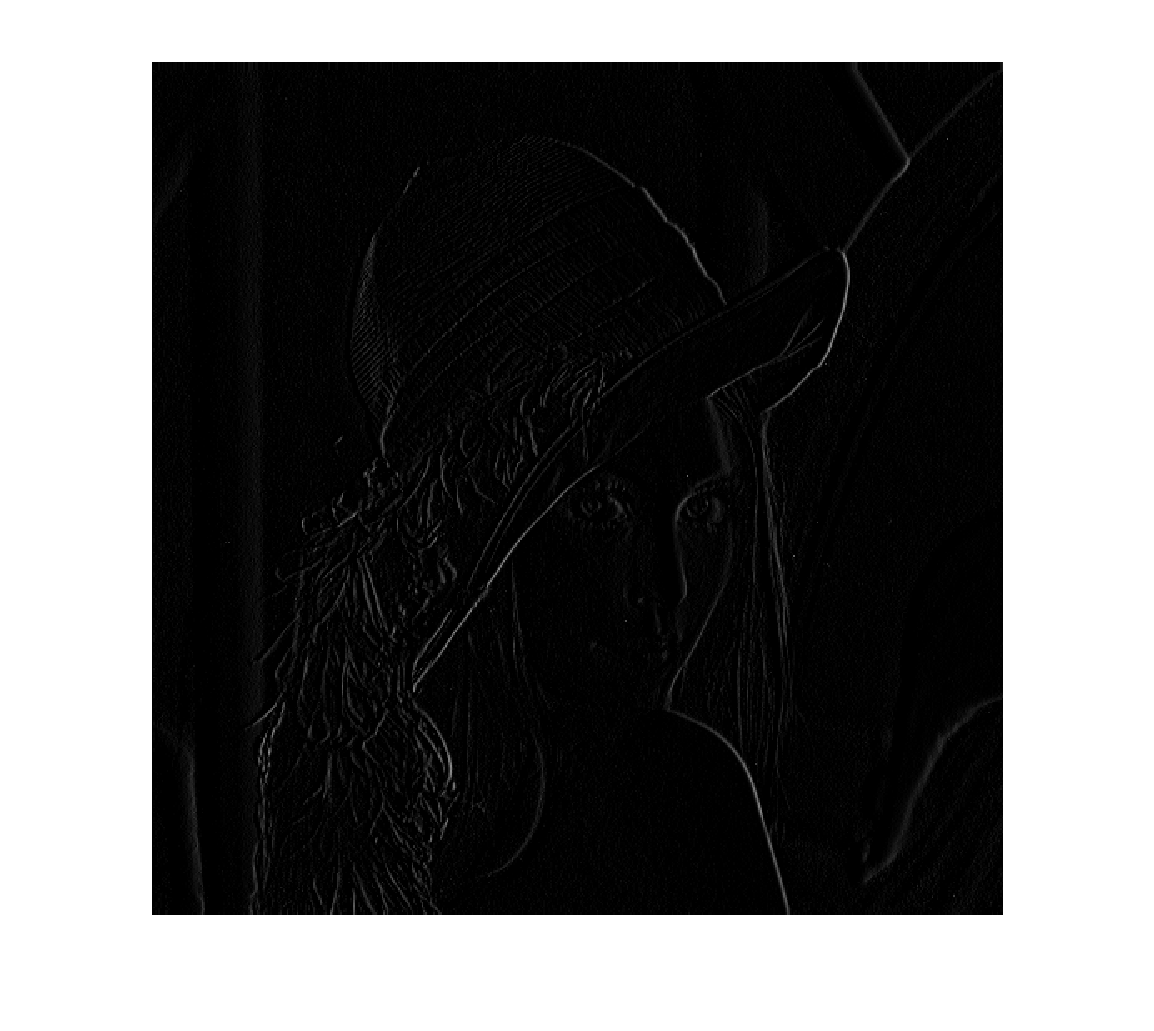
\includegraphics[width=\textwidth]{images/conv1}
                \caption{myconv.}
                \label{fig:myconv}
        \end{subfigure}
        \begin{subfigure}[b]{0.32\textwidth}
                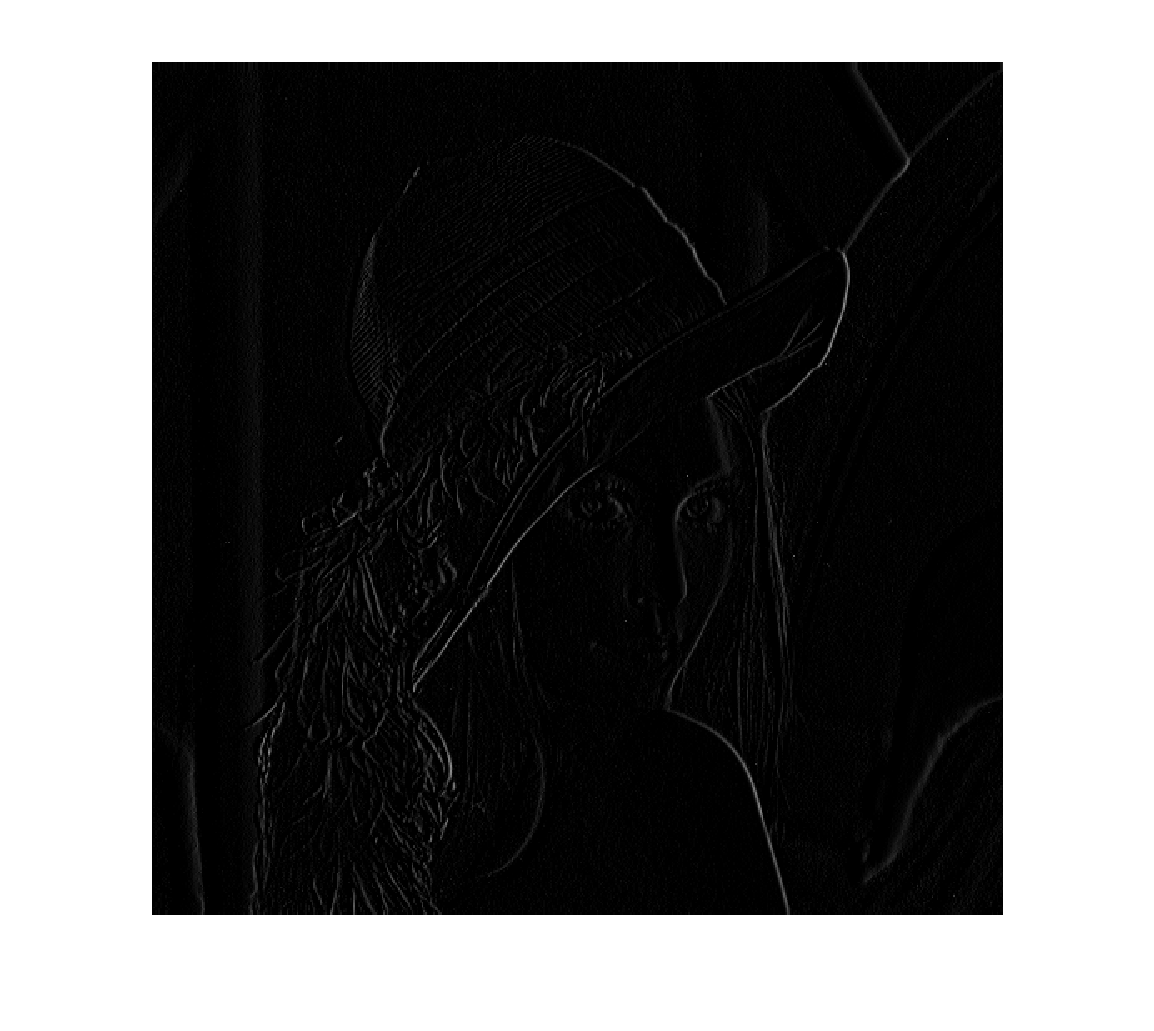
\includegraphics[width=\textwidth]{images/conv2}
                \caption{myconvFFT.}
                \label{fig:myconvFFT}
        \end{subfigure}
        \begin{subfigure}[b]{0.32\textwidth}
                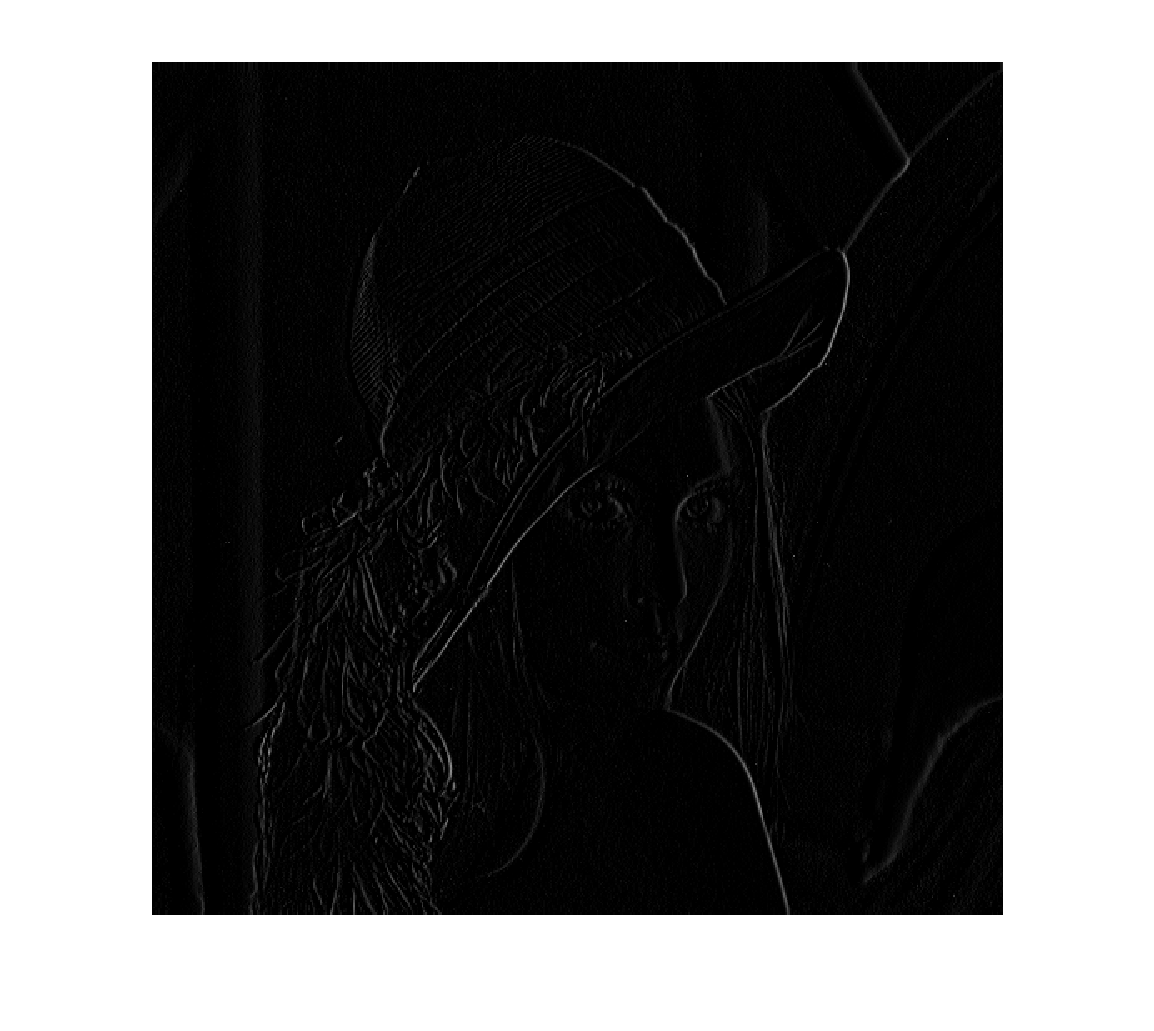
\includegraphics[width=\textwidth]{images/conv2}
                \caption{Matlab's conv2.}
                \label{fig:conv2}
        \end{subfigure}
        \caption{Comparative of the different convolution codes with a horizontal sovel kernel $k = \left[-1, 1 \right]$.}\label{fig:convolution}
\end{figure}

\begin{table}[h]
	\centering
	\begin{tabular}{|c|c|c|c|}
	\hline
     & myconv & myconvFFT & Matlab's conv2 \\ \hline
	Time & 0.658s   & 0.04s     & 0.002s   \\ \hline
	\end{tabular}
	\caption{Performance comparative of the convolution methods.}
	\label{tb:convolutionPerfomance}
\end{table}
 
In Figure~\ref{fig:convolution} we see that the convolution theorem holds, and in Table~\ref{tb:convolutionPerfomance} that performing the operations in the Fourier domain and transforming back is more efficient.

\section{Features}

Being able to detect features in images that are invariant to rotations, translations, scale and changes in illumination is an useful tool, with many applications such as image matching.
SIFT features, proposed by \cite{Lowe2004}, provide a fairly robust method to detect points in an image with the aforementioned restrictions.
A broad overview of the algorithm is:
\begin{enumerate}
\item \textbf{Extrema detection:} maximum and minimum intensity points are detected in a difference-of-Gaussian pyramid built with the input image.
\item \textbf{Keypoint refinement:} point centrer in interpolated and weak points are rejected.
\item \textbf{Orientation assignment:} orientation and strength of each keypoint are calculated.
\item \textbf{Descriptor calculation:} a 128 feature vector is computed for every element.
\end{enumerate}

\begin{figure}[htbp]
	\centering
	\begin{minipage}[t]{.48\textwidth}
		\centering
		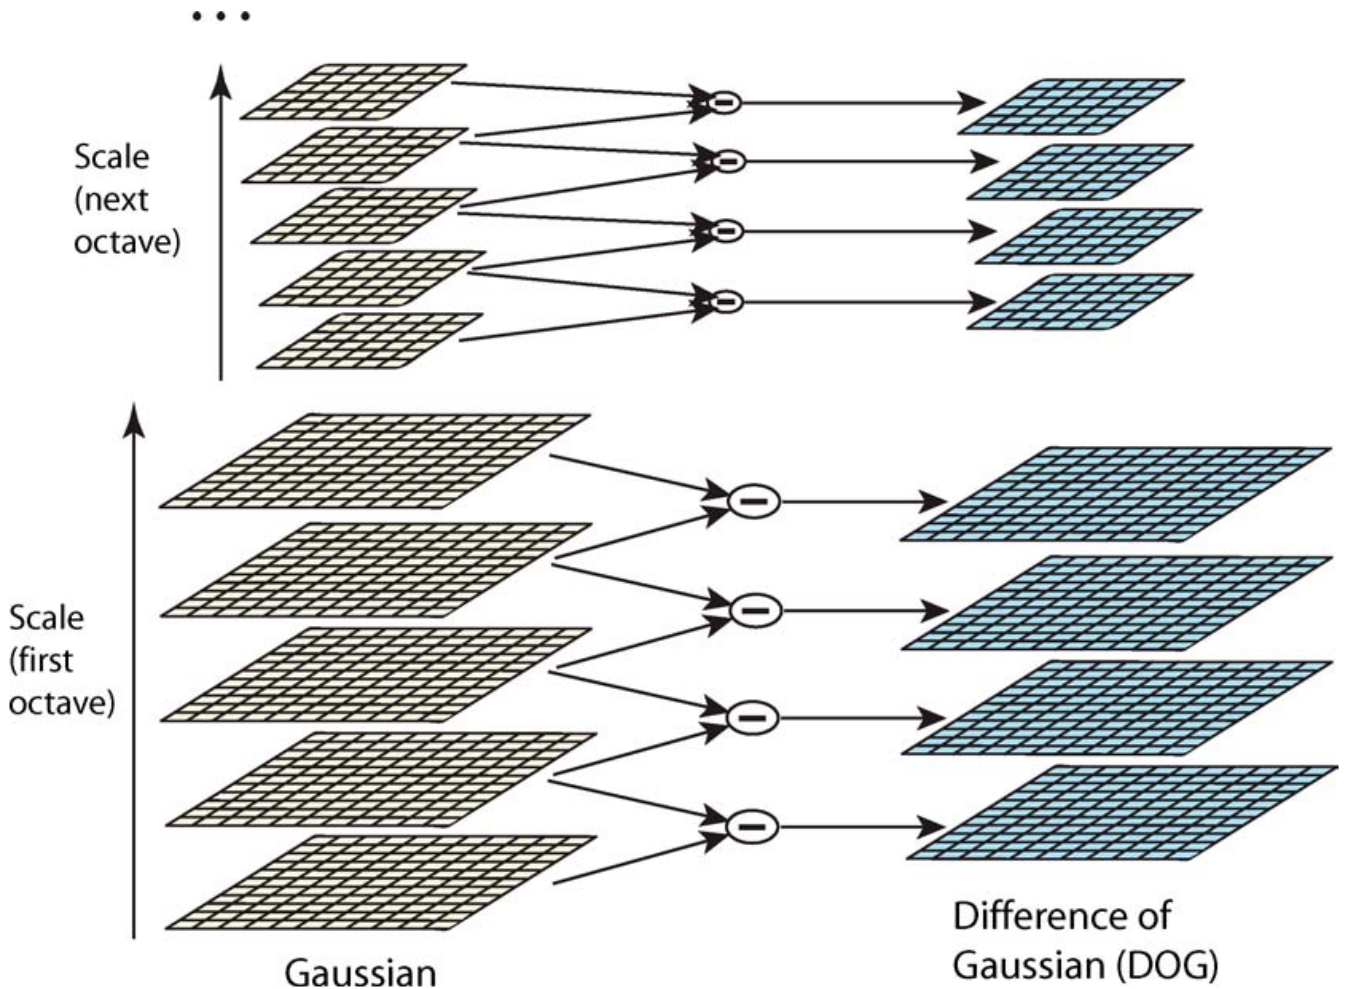
\includegraphics[width=1.05\textwidth]{images/diffOfGauFromPaper}
		\caption{Pyramid of difference-of-Gaussian, \cite{Lowe2004}.}
		\label{fig:difOfGauPyramid}
	\end{minipage} ~
	\begin{minipage}[t]{.48\textwidth}
		\centering
		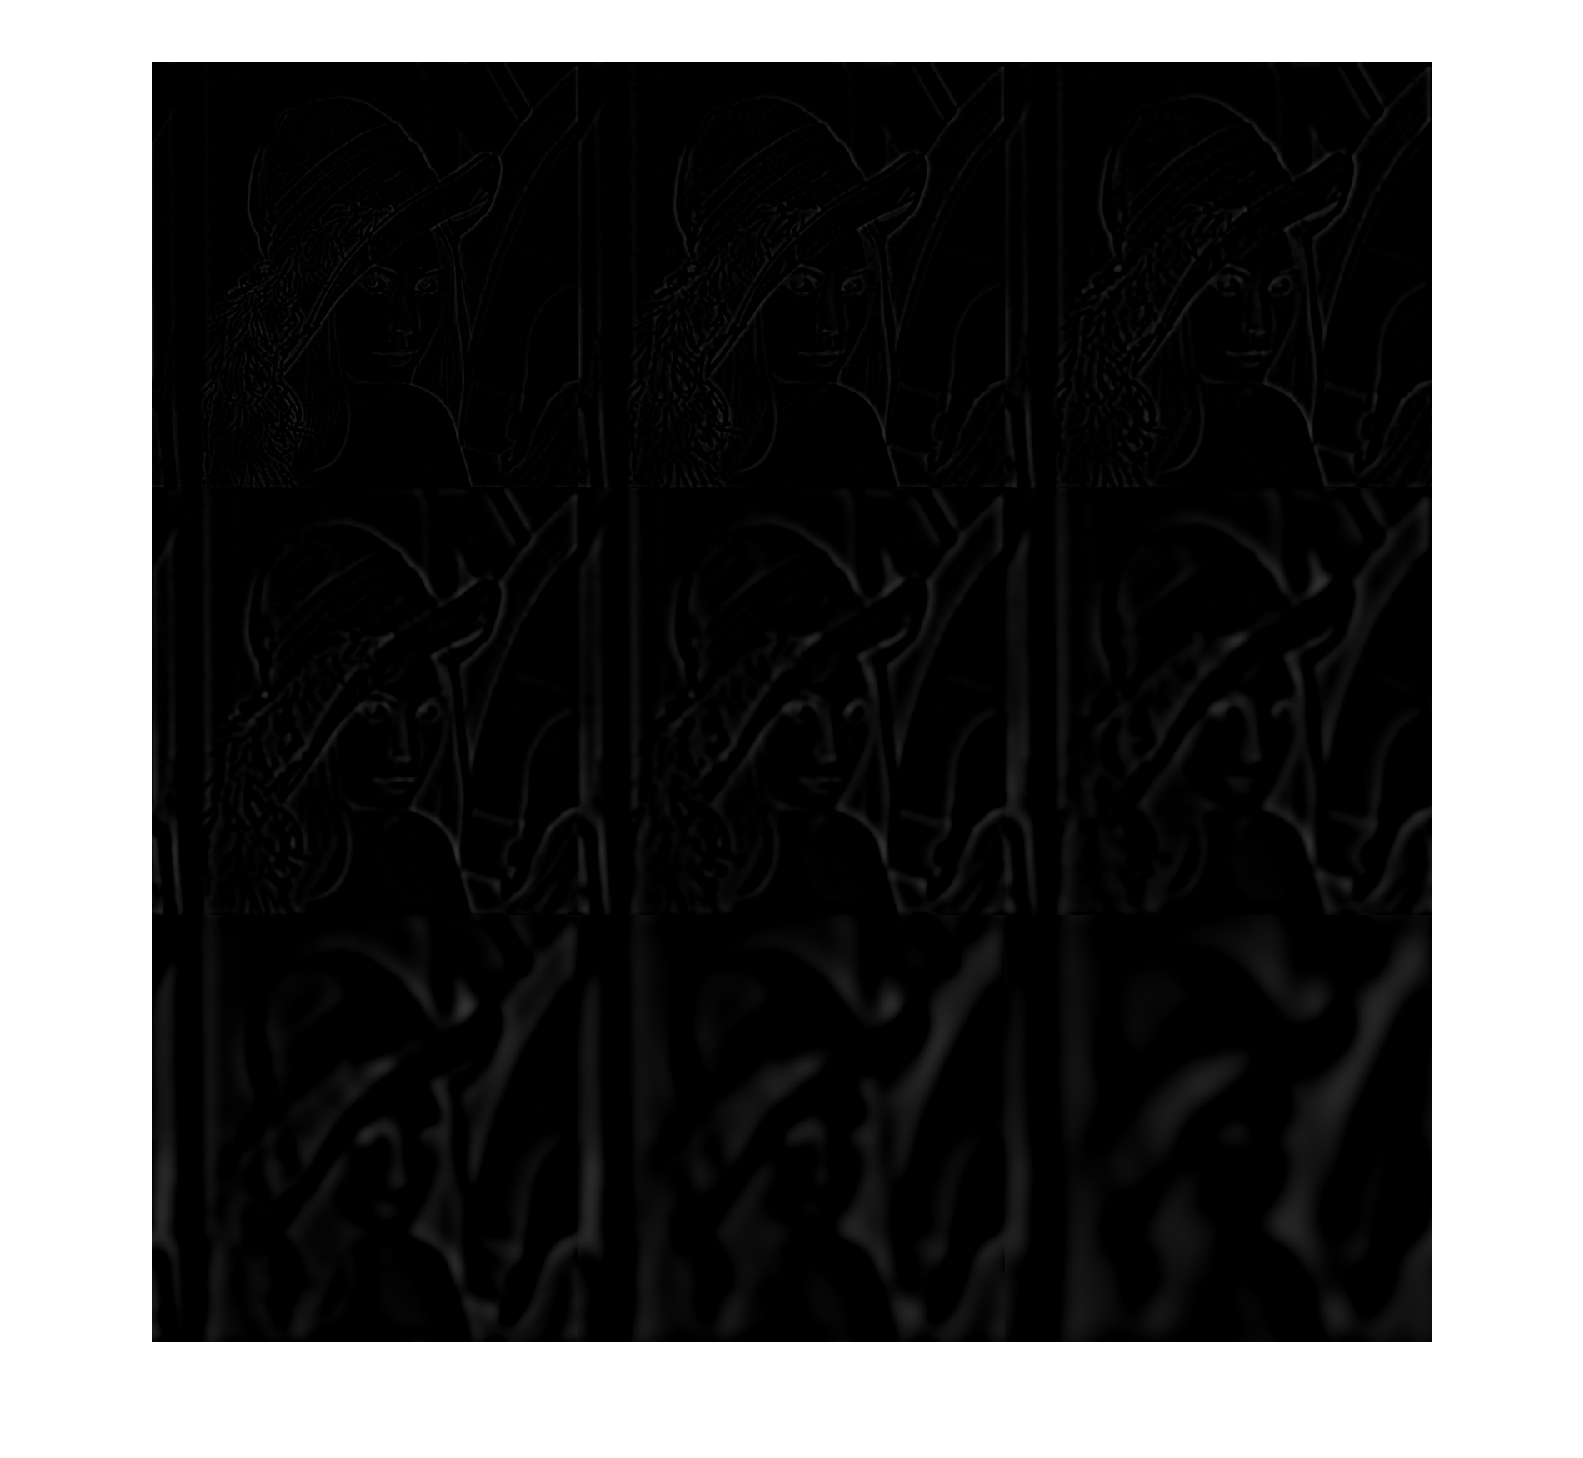
\includegraphics[width=1\textwidth]{images/dogSpace}
		\caption{Example of a scale of a difference-of-Gaussian.}
		\label{fig:difOfGauSample}
	\end{minipage}
\end{figure}

\textbf{Extrema detection} is computed using a difference-of-Gaussian (DOG) structure, as shown in Figure~\ref{fig:difOfGauPyramid}, first a scale of blurred images is constructed.
The input image $I$ is convoluted with a Gaussian kernel $G$:

\begin{equation}
L(x,y,\sigma) = G(x,y,\sigma) * I(x,y),
\end{equation}

where $L$ is the output image, $*$ the convolution operator, $x$ and $y$ the pixel indices, and $G$ and Gaussian kernel defined as:

\begin{equation}
G(x,y,\sigma) = \frac{1}{2 \pi \sigma^2} e^{- \frac{x^2 + y^2}{2 \sigma^2}},
\end{equation}

where $\sigma$ is the standard deviation.
Next, the DOG structure is computed as a difference of several $L$:

\begin{equation}
D(x,y,\sigma) = L(x,y, k\sigma) - L(x,y, \sigma),
\end{equation}

where $D$ is the output image and $k$ is a constant multiplicative factor.
Note that to provide an efficient implementation, the convolution and difference can be computed in the Fourier domain using the convolution theorem explained in Section~\ref{sec:convolution}.
A example on how this DOG structure looks like is shown in Figure~\ref{fig:difOfGauSample}, where the sigma increases from left to right and from top to bottom.
The keypoints selected will be those who are a maximum or a minimum in a $3 \times 3 \times 3$ cube region, so in their scale and the ones above and below.
Selecting locations using this scheme allows to find interested points regardless of their scale, as we progress towards the top of the pyramid,  the local maximum or minima will be produced by bigger objects in $I$.
In our implementation only one scale of the pyramid is calculated.

Keypoint refinement is done with an optimization step which removes weak points and also improves their position.
The new keypoint location $\mathbf{\hat{x}}$ will be:

\begin{equation}
\mathbf{\hat{x}} = - \frac{\partial^2 D^{-1}}{\partial \mathbf{x^2}} \frac{\partial D}{\partial \mathbf{x}},
\end{equation}

where $\mathbf{x}$ is the previous location and $D(\mathbf{x})$ is approximated with a Taylor expansion in the form of:

\begin{equation}
D(\mathbf{x}) = D + \frac{ \partial D^T}{\partial \mathbf{x}} \mathbf{x} + 0.5 \mathbf{x}^T \frac{\partial^2 D}{\partial \mathbf{x^2}}\mathbf{x}.
\end{equation}

Keypoints are rejected if they are weak or in an edge, any extrema is defined as weak if $D(\mathbf{x}^T) < 0.03$, where $D(\mathbf{\hat{x}})$ is:

\begin{equation}
D(\mathbf{\hat{x}}) = D + 0.5 \frac{\partial D^T}{\partial \mathbf{x}}\mathbf{\hat{x}}.
\end{equation}

Edge elimination is performed when $R(\mathbf{H}) > f(r)$, where $\mathbf{H}$ is a $2 \times 2$ Hessian matrix, $r = 10$, $R(\mathbf{H})$ is defined as:

\begin{equation}
R(\mathbf{H})= \frac{ (D_{xx} + D_{yy})^2 }{ D_{xx} D_{yy} - (D_{xy})^2} ~ \text{where} ~ D_{\alpha \beta} = \frac{\partial^2 D}{\partial \alpha \partial \beta} ~  \text{for} ~ \alpha, \beta = x, y
\end{equation}

and 

\begin{equation}
f(r) = \frac{(r + 1)^2}{r}.
\end{equation}

\textbf{Orientation assignment} measures the point orientation using local images properties.
The objective is that if a point is rotated in another image, the final descriptor will be the same in both.
A gradient magnitude $m(x,y)$ and orientation angle $\theta(x,y)$ are computed as follows:

\begin{equation}
\begin{aligned}
	m(x,y) &= \sqrt[]{(L(x+1,y,\sigma) - L(x-1,y,\sigma))^2 + (L(x,y+1,\sigma) - L(x,y-1,\sigma))^2}, \\
	\theta(x,y) &= tan^{-1} \left( \left( L(x,y+1,\sigma) - L(x, y-1, \sigma) \right) / \left( L(x+1,y,\sigma) - L(x-1, y, \sigma) \right) \right),
\end{aligned} \label{eq:conv}
\end{equation}

where $L$ is chosen to has the same sigma as the keypoint.

\textbf{Descriptor calculation} uses orientation histograms from sample points near the extrema.
For each keypoint a $16 \times 16$ region around it is chosen and the orientations for each pixel are calculated.
$4 \times 4$ histograms are computed with 8 bins each; this 8-dimensional values are placed in an array forming a 128 element feature vector for each keypoint.
Normalizing the vector to unit length improves invariance to illumination changes.

%\begin{figure}[htbp!]
%        \centering
%        \begin{subfigure}[b]{0.45\textwidth}
%                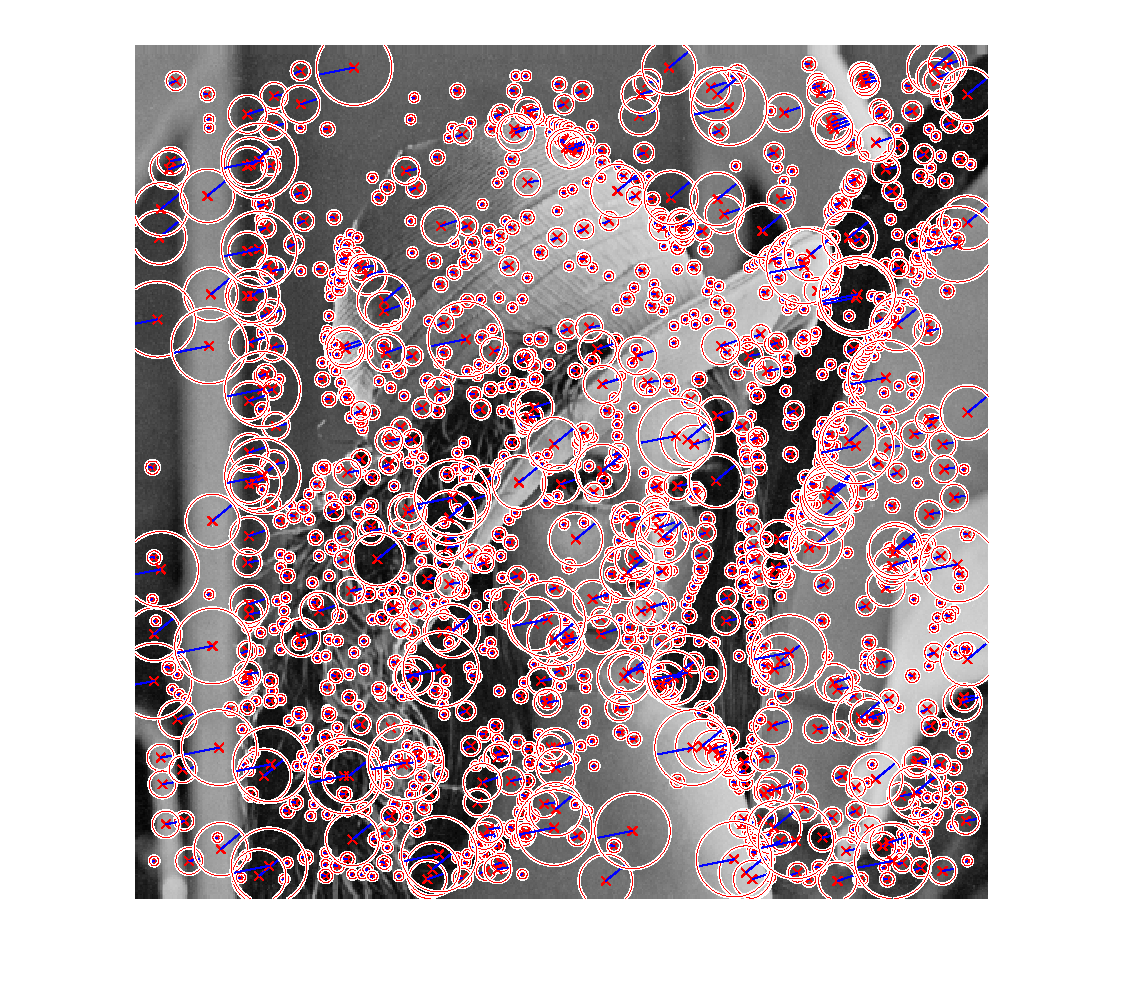
\includegraphics[width=\textwidth]{images/sift2}
%                \caption{SIFT without weak and edge keypoint purge.}
%                \label{fig:sift1}
%        \end{subfigure}
%        \begin{subfigure}[b]{0.45\textwidth}
%                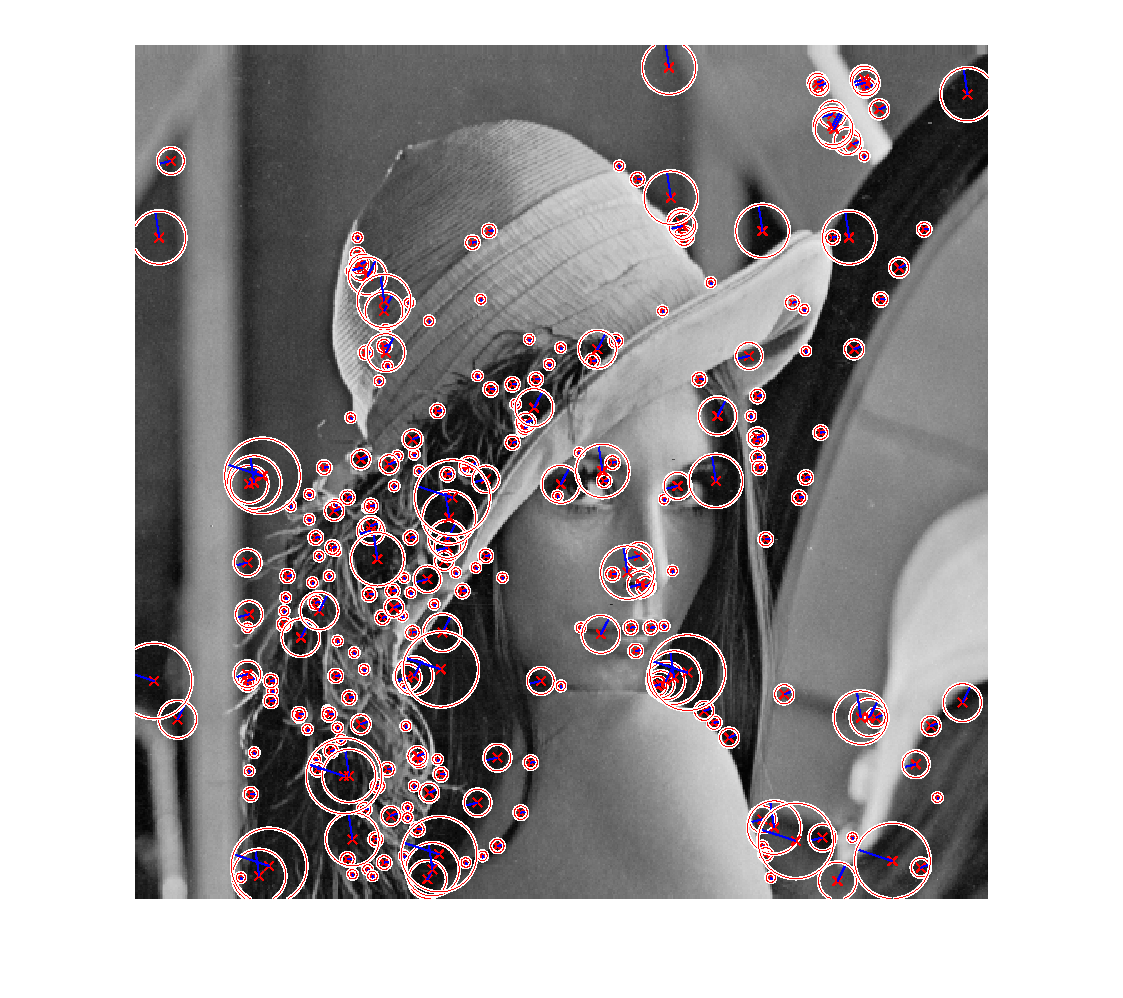
\includegraphics[width=\textwidth]{images/sift1}
%                \caption{SIFT with weak and edge keypoint removal.}
%                \label{fig:sift2}
%        \end{subfigure}
%        \begin{subfigure}[b]{0.45\textwidth}
%                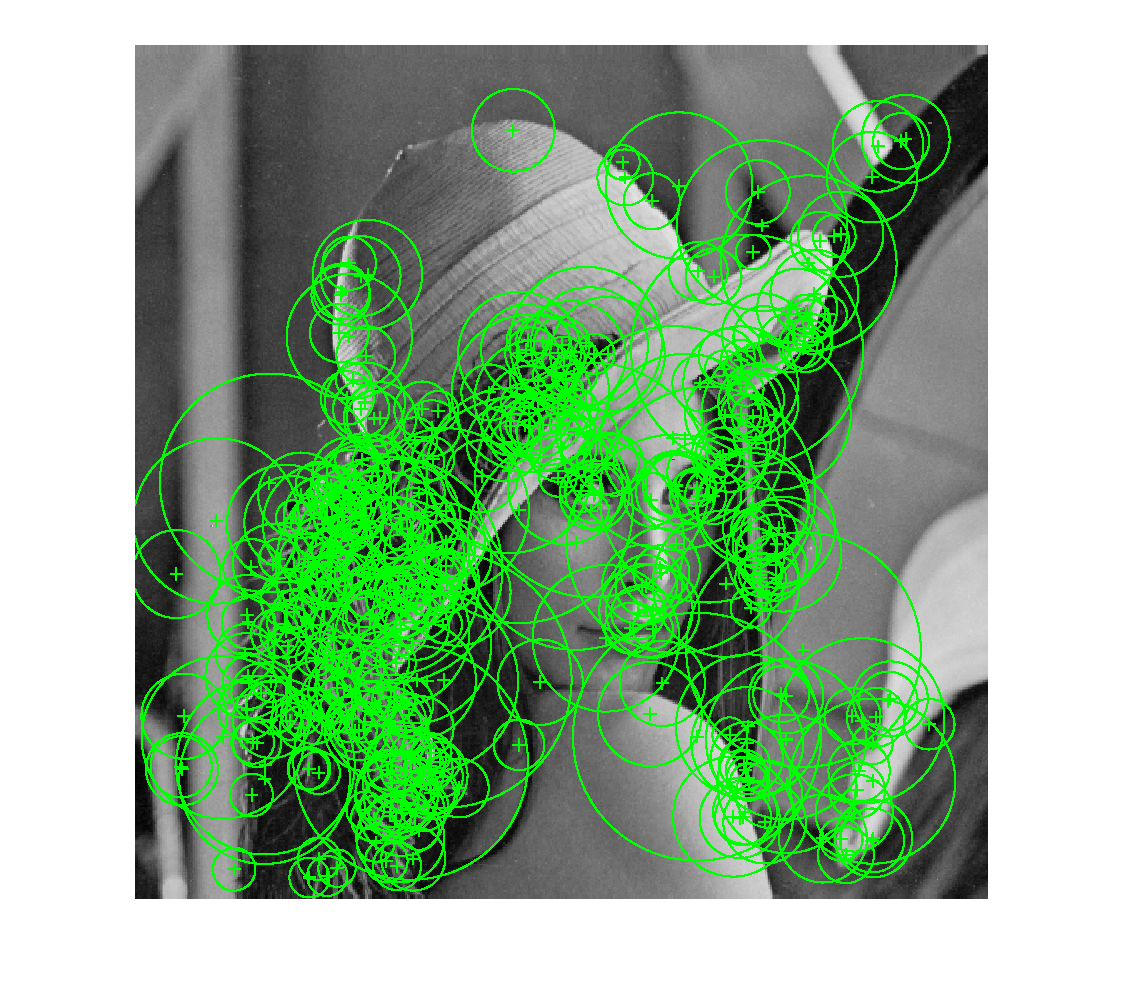
\includegraphics[width=\textwidth]{images/surf1}
%                \caption{SURF with default parameters.}
%                \label{fig:surf1}
%        \end{subfigure}
%        \begin{subfigure}[b]{0.45\textwidth}
%                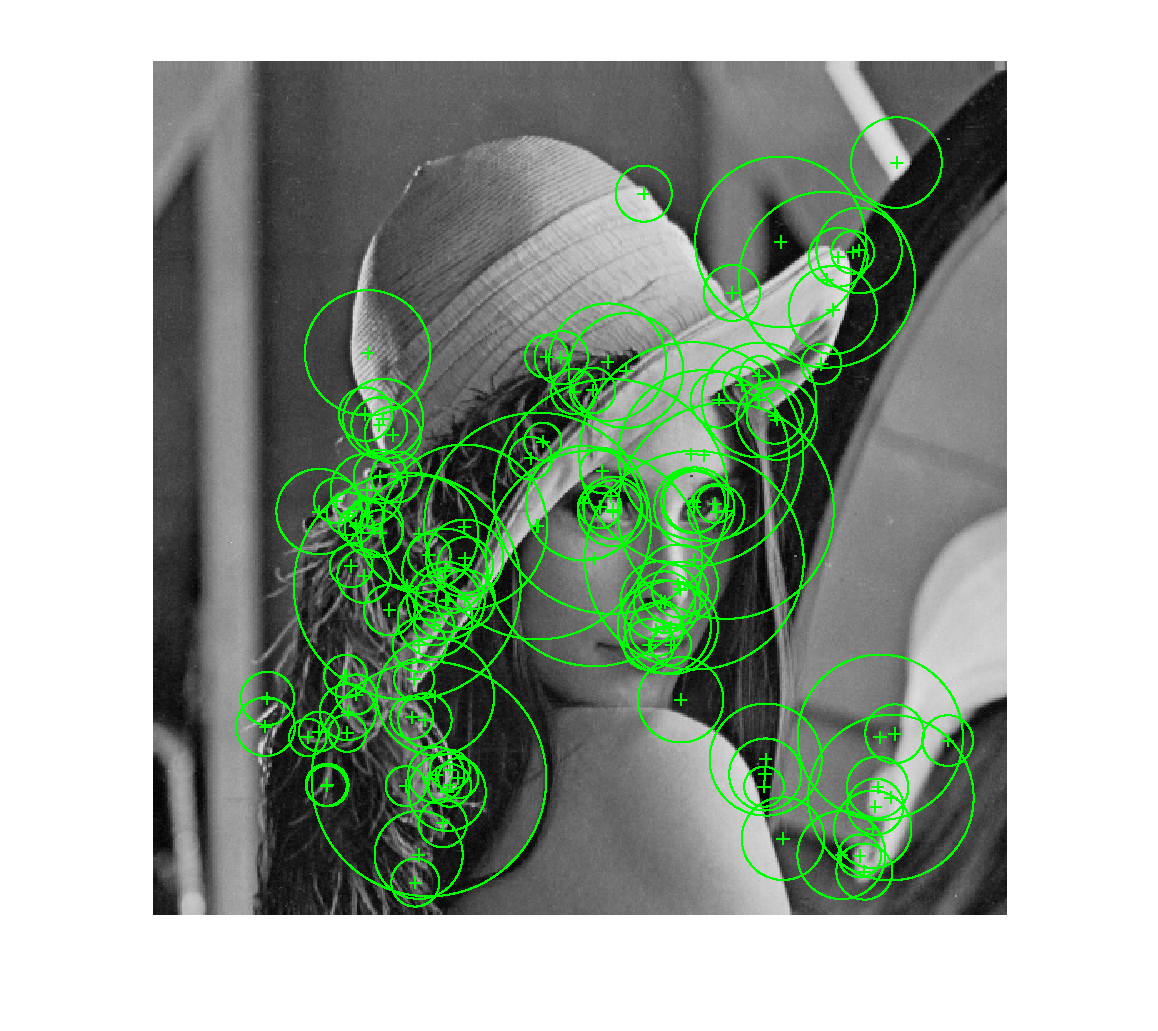
\includegraphics[width=\textwidth]{images/surf2}
%                \caption{SURF with the 120 strongest keypoints.}
%                \label{fig:surf2}
%        \end{subfigure}        
%        \caption{Comparative of our SIFT features with Matlab's SURF features.}\label{fig:featuresSample}
%\end{figure}

\FloatBarrier % Makes sure the previous figure does not go into the Matching section
\section{Matching}

In the image matching area an image $I_0$ is to be found under a certain affine transformation in another image $I_1$.
Due to camera measurement errors, changes in illumination and other factors, a global optimal solution is computationally expensive.
The RANSAC (Random Sample Consensus) algorithm is a simple and fast approach to perform this task, \cite{Fischler1981}.
Despite being originally designed to estimate the parameters that fit a mathematical model to a dataset which contains outliers, it can also be used to estimate the transformation $H$ that matches $I_0$ and $I_1$.
A general overview of the algorithm is given below:

\begin{algorithm}[H]
 \caption{RANSAC}
 \KwData{A pair of images $I_0$ and $I_1$, $k$ number of iterations, distance threshold $t$.}
 \KwResult{Homography matrix $H$.}
 $f_0$, $f_1$ = detectKeypoints($I_0$, $I_1$)\;
 $m$ = matchFeatures($f_0$, $f_1$)\;
 $H = identity$\;
 \For{$i\leftarrow 0$ \KwTo $k$ }{
  $rp$ = pickRandomPoints($m$)\;
  $newH$ = computeHomography($rp$)\;
  \If{$newH$ is better than $H$}{
   $H = newH$\;
   }
 }
\end{algorithm}

To detect and match the keypoints, our implementation uses SURF features CITATION.
We want to calculate the matrix $H$ that transforms from one image to the other, such that:

\begin{equation}
\begin{bmatrix}
u \\ 
\vv \\ 
w
\end{bmatrix}
= 
\begin{bmatrix}
 h_{11} & h_{12} & h_{13} \\ 
 h_{21} & h_{22} & h_{23}\\ 
 h_{31} & h_{32} & h_{33}
\end{bmatrix}
\begin{bmatrix}
u' \\
\vv' \\
w'
\end{bmatrix},
\label{eq:originalH}
\end{equation}

where $u$, $\vv$ and $w$ are the scaled pixel coordinates in $I_1$ and $u'$, $\vv'$ and $w'$ the scaled pixel coordinates in $I_0$.
Collecting $H$ in rows, $H_i = \begin{bmatrix} h_{i1} & h_{i2} & h_{i3} \end{bmatrix}$ for $i = \lbrace 1,2,3 \rbrace$ and $\mathbf{u'} = \begin{bmatrix} u' & \vv' & w' \end{bmatrix}$ we can rewrite Equation~\ref{eq:originalH} into:

\begin{equation}
\begin{aligned}
	u = H_1 \mathbf{u'}, \: \vv &= H_2 \mathbf{u'}, \: w = H_3 \mathbf{u'}, \\ 
	\text{enforcing} \: w &= 1, \\
	u^* = \frac{H_1 \mathbf{u'}}{ H_3 \mathbf{u'}}, \: \vv^* &= \frac{H_2 \mathbf{u'}}{ H_3 \mathbf{u'}}, \: \text{hence} \\	
	%
	u^*H_3\mathbf{u'} - H_1\mathbf{u'} &= 0, \\
	\vv^* H_3\mathbf{u'} - H_2\mathbf{u'} &= 0, \: thus\\
	%
	\begin{bmatrix}
	-\mathbf{u'} & \mathbf{0} & u^*\mathbf{u'} \\
	\mathbf{0} & -\mathbf{u'} & \vv^*\mathbf{u'}
	\end{bmatrix}
	%
	\begin{bmatrix}
	H_1^T \\
	H_2^T \\ 
	H_3^T 
	\end{bmatrix}
	&= \mathbf{0}^T,
\end{aligned}
\label{eq:derivatingH}
\end{equation}

where $\mathbf{0} = \begin{bmatrix} 0 & 0 & 0 \end{bmatrix}$. 
As shown above, each match provides two equations to solve $H$.
Since, we enforce the scale to be a homogeneous coordinate, $h_{33} = 1$ is no longer an unknown.
For eight unknowns, eight equations are needed, so four points in each image are to be matched.
In matrix notation, we will stack all the equations in a matrix $A$, such that $A\mathbf{h}=0$, where $\mathbf{h}$ is $H$ reshaped into a column vector.
Singular value decomposition of $A$ can be computed to solve the system, $A = UZV^T$, where $U$ and $V$ are unitary, $Z$ is rectangular diagonal and $\mathbf{h} = V_{i9}$ for $i = \lbrace 1,2, \ldots, 9 \rbrace$.

The metric to define if a $newH$ is better than a previously calculated $H$ is double; each match keypoint in $I_0$ is transformed with $newH$, the euclidean distance from the matched point in $I_1$ is calculated, and if it is below a threshold $t$, we count it as a good match.
$newH$ is considered an improvement over $H$, if it produces more good matches than $H$ or the same number although with lower error.
Some results obtained with our code are shown in Figure~\ref{fig:ransacSample}.

\begin{figure}[htbp!]
        \centering
        \begin{subfigure}[b]{0.7\textwidth}
                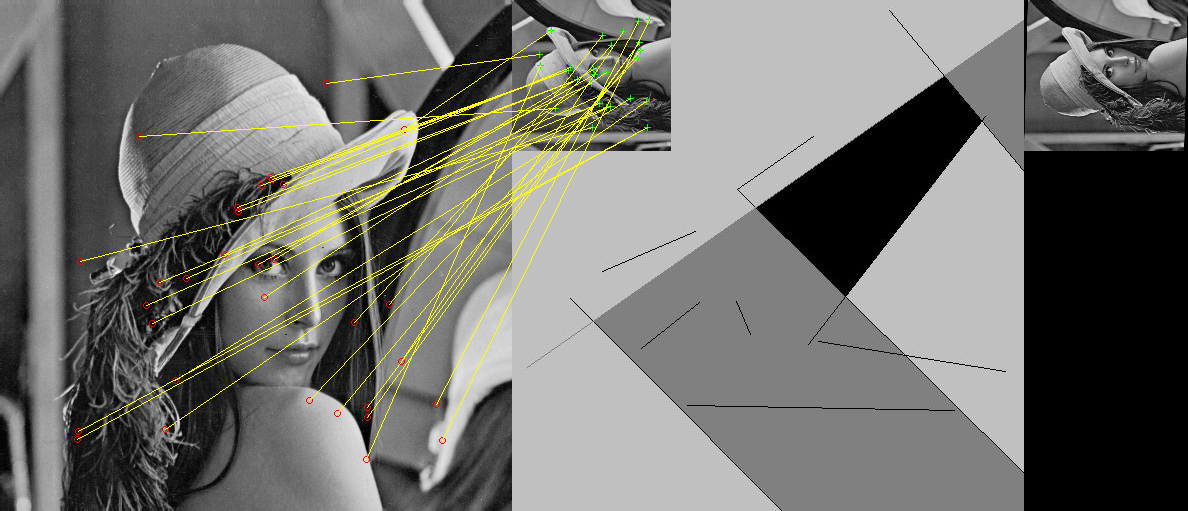
\includegraphics[width=\textwidth]{images/ransac2}
                \caption{A synthetic test.}
                \label{fig:ransac1}
        \end{subfigure}    
        \begin{subfigure}[b]{0.7\textwidth}
                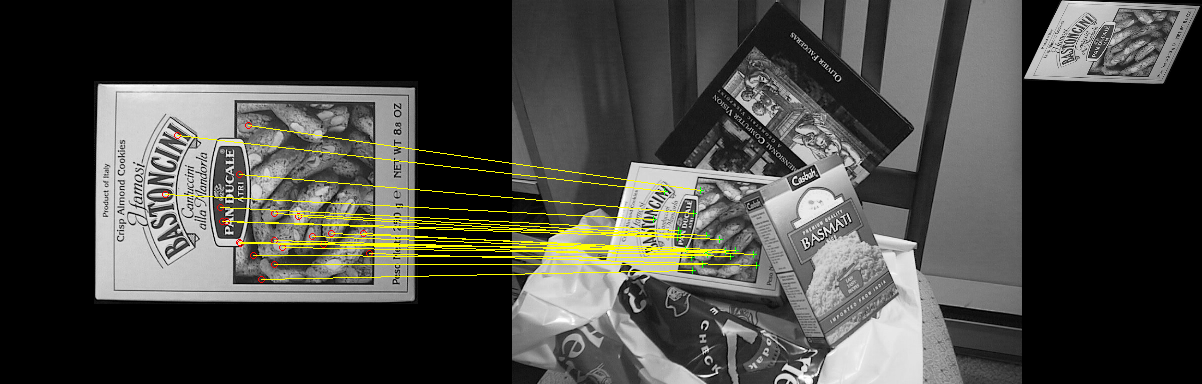
\includegraphics[width=\textwidth]{images/ransac1}
                \caption{Matching a box, images taken from \cite{Lowe2004}.}
                \label{fig:ransac2}
        \end{subfigure} 
        \caption{Samples of $H$ computation, left is $I_0$, centre is $I_1$ and right is $I_0 * H$. Keypoints matching between input images is shown for clarity.}\label{fig:ransacSample}
\end{figure}

\FloatBarrier
\section{Reconstruction}

3D stereo reconstruction from a par of cameras involves three steps:
\begin{enumerate}
\item \textbf{Camera calibration:} compute camera model parameters.
\item \textbf{Fundamental matrix:} estimate an $F$ matrix such that $\mathbf{u}'^TF\mathbf{u} = 0$, where $\mathbf{u}$ and $\mathbf{u}'$ are corresponding points in two images.
\item \textbf{Reconstruct 3D points:} once constrained by $F$, triangulate points position from the two images.
\end{enumerate}

We will model our cameras using the pinhole camera model, in this framework a world 3D point $\mathbf{x} = \begin{bmatrix} x & y & z & 1 \end{bmatrix}$ is projected into a 2D image point $\mathbf{u} = \begin{bmatrix} u & \vv & 1 \end{bmatrix}$ using the following equations:

\begin{gather}
	\mathbf{u}^T = P \mathbf{x}^T, \label{eq:matrixP} \\
	\mathbf{u}^T = K [R | \mathbf{t}] \mathbf{x}^T, \label{eq:matrixRT}
\end{gather}

where $K$ is 
\begin{equation}
\begin{bmatrix}
f_x & 0 & p_x \\ 
0 & f_y & p_y \\ 
0 & 0 & 1
\end{bmatrix}
\end{equation}

with $f_x$ and $f_y$ are focal length parameters and $p_x$ and $p_y$ is the principal point, $P$ is a $3 \times 4$ projection matrix, $R$ is a $3 \times 3$ rotation matrix, $t$ is a translation column vector, making $[R|t]$ a $3 \times 4$ matrix.
Note that $\mathbf{x}$ and $\mathbf{u}$ have a homogeneous coordinate.
$K$ and $[R|\mathbf{t}]$ is commonly referred as camera intrinsics and extrinsics matrix respectively, and the estimation of their elements is known as \textbf{camera calibration}.

Equation~\ref{eq:matrixP} can be solved following equivalent steps as to those used in Equations~\ref{eq:originalH} and~\ref{eq:derivatingH}, although with an extra coordinate in $\mathbf{x}$ and regarding $P$ as equivalent to $H$ with an added column.
Therefore we can again stack several points in a matrix $A$, yet the increased number of unknowns determine that six points are needed to estimate $P$:

\begin{equation}
A\mathbf{p} = 0.
\end{equation}

Once we have solved the aforementioned equation with SVD, we need to decompose $P$ into $K[R|t]$.
Since $K$ is an upper triangular matrix, we can use an a $RQ$ decomposition on $P$, where $R$ is upper triangular and $Q$ is orthogonal, \cite{Francis1961}.
For the decomposition only the first three columns in $P$ will be used, and $\mathbf{t} = K^{-1}P_4$, where $P_4$ is the last column in $P$.

% Figure with calibration object???

\begin{figure}[htbp!]
	\centering
	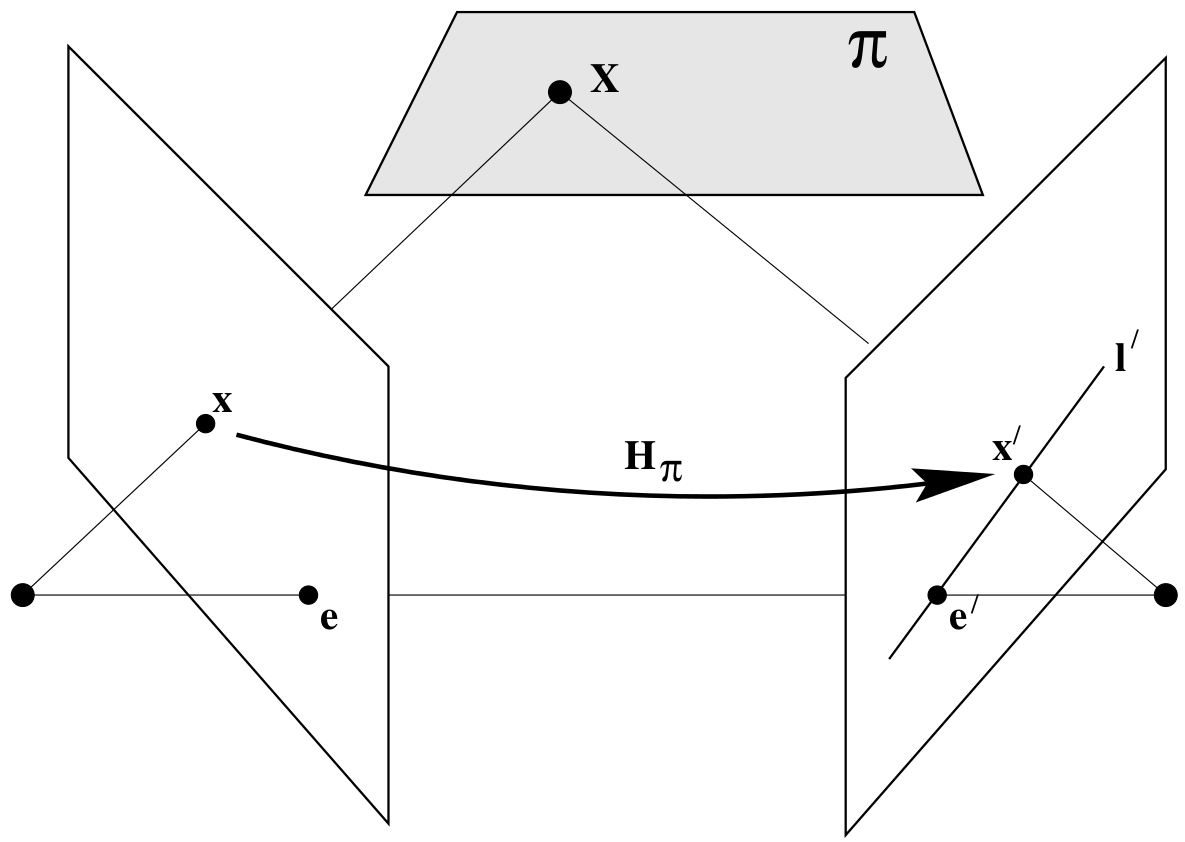
\includegraphics[width=0.4\textwidth]{images/epipolarLines}
	\caption{A point $\mathbf{x}$ in the left image is mapped via a plane $\boldsymbol{\pi}$ to a point $\mathbf{x}'$ in the right image.}\label{fig:epipolarLines}
\end{figure}

Epipolar lines and the \textbf{fundamental matrix} $F$ are useful tools in stereo reconstruction.
In Figure~\ref{fig:epipolarLines} the geometrical relation of the projection a 3D world point $\mathbf{X}$ in two cameras is shown.
We define $\mathbf{e}$ and $\mathbf{e}^T$ as the epipolar points (epipoles), $F$ is a matrix that satisfies $\mathbf{u}'^TF\mathbf{u} = 0$, where $\mathbf{u} = \begin{bmatrix} u & \vv & 1 \end{bmatrix}$ and $\mathbf{u}' = \begin{bmatrix} u' & \vv' & 1 \end{bmatrix}$ are matching points in the left and right images respectively, and $\mathbf{l}^T$ is a line such that $\mathbf{l}^T = F\mathbf{x}$.

To calculate $F$ an approach in Equations~\ref{eq:originalH} and~\ref{eq:derivatingH} can be used again.
However, in the equation $A\mathbf{f} = 0$, this time $A$ will have following configuration:

\begin{equation}
\begin{bmatrix}
u_1 u_1' & 	\vv_1 u_1' & u_1' & u_1 \vv_1' & \vv_1 \vv_1' & \vv_1' & u_1 & \vv_1 & 1 \\
\vdots & \vdots & \vdots & \vdots & \vdots & \vdots & \vdots & \vdots & \vdots  \\
u_8 u_8' & \vv_8 u_8' & u_8' & u_8 \vv_8' & \vv_8 \vv_8' & \vv_8' & u_8 & \vv_8 & 1 
\end{bmatrix}
\begin{bmatrix}
F_1^T \\
F_2^T \\
F_3^T \\
\end{bmatrix}
= \mathbf{0}^T,
\end{equation}

where the $\mathbf{f}$ is $F$ reshaped in a column vector and the $l$ and $r$ indices represent points from the left and right images respectively; $F$ can be estimated using SVD.

Since we have calculated all the necessary parameters for each camera and their relationship, we can now proceed to stereo reconstruction.
Below a possible implementation in pseudocode in presented:

\begin{algorithm}[H]
 \caption{Stereo Reconstruction}
 \KwData{A pair of images $I_0$ and $I_1$, projection matrices for two cameras $P_0$ and $P_1$.}
 \KwResult{Cloud of 3D points $\mathbf{X}$.}
 $f_0$, $f_1$ = detectKeypoints($I_0$, $I_1$)\;
 $m$ = matchFeatures($f_0$, $f_1$)\;
 \For{$i\leftarrow 1$ \KwTo $numMatches$ }{
	$A$ = constructA($m(i)$)\;
	$X(i)$ = SVD($A$)\;
 }
 displayCloud(X)\;
\end{algorithm}

For this task we have a set of correspondences:

\begin{equation}
 \mathbf{u}_{i} = P\mathbf{x}_i, \quad \mathbf{u'}_{i} = P'\mathbf{x}_i,
\end{equation}

where the unknown is the 3D world object position $\mathbf{x}_i$.
Solving for a single point $\mathbf{x}$, we cluster the rows of $P$, such as $P_i = \begin{bmatrix} p_{i1} & p_{i2} & p_{i3} & p_{i4}  \end{bmatrix}$ for $i = \lbrace 1, 2, 3 \rbrace$,

\begin{equation}
 u = P_1\mathbf{x}, \quad \vv = P_2\mathbf{x}, \quad 1 = P_3\mathbf{x},\\
\end{equation}

multiplying the first and second equation by the third,

\begin{equation}
\begin{aligned}
	uP_3\mathbf{x} &=  P_1\mathbf{x} \: \rightarrow  \: uP_3\mathbf{x} - P_1\mathbf{x} = 0,\\
	\vv P_3\mathbf{x} &= P_2\mathbf{x} \: \rightarrow \: \vv P_3\mathbf{x} - P_2\mathbf{x} = 0,
\end{aligned}
\end{equation}

doing the equivalent for the right camera equation and stacking the result below the left one,

\begin{equation}
	\begin{bmatrix}
	uP_3 - P_1 \\
	\vv P_3 - P_2 \\
	u'P_3' - P_1' \\
	\vv' P_3' - P_2'	
	\end{bmatrix}
	%
	\mathbf{x}^T
	= \mathbf{0}^T \: \rightarrow  \: A\mathbf{x}^T = \mathbf{0}^T.
\end{equation}

We can calculate $\mathbf{x}$ via singular value decomposition; for each point $\mathbf{x}_i$ a new $A_i$ matrix will be compute and the system will be solved.
Our implementation extracts the matches using SURF keypoints, however this produces a sparse reconstruction as only a small subset of points in the image is matched.
In Figure~\ref{fig:stereoReconstruction} the reconstruction results are shown.
The scene (modelled using Blender) contains some books on a self with a textured plane on the background, based on \cite{Archemi2014}.
The cameras position can be seen on the upper sections of Figures~\ref{fig:blender1} and~\ref{fig:blender2}.
The matching algorithm produces 87 points in this example, however only 75 are rendered due to some erroneous matches being discarded.
Some details can be seen in Figure~\ref{fig:stereoRecons2}, the two blue circles depict both cameras position; the cloud has three distinctive clusters, the left one shows the points one the background, the centre-top one represents the points on the cover of the books, and the line-shaped cluster below the books, displays the points tracked on the background under the shelf.

\begin{figure}[htbp]
        \centering
        \begin{subfigure}[b]{0.32\textwidth}
                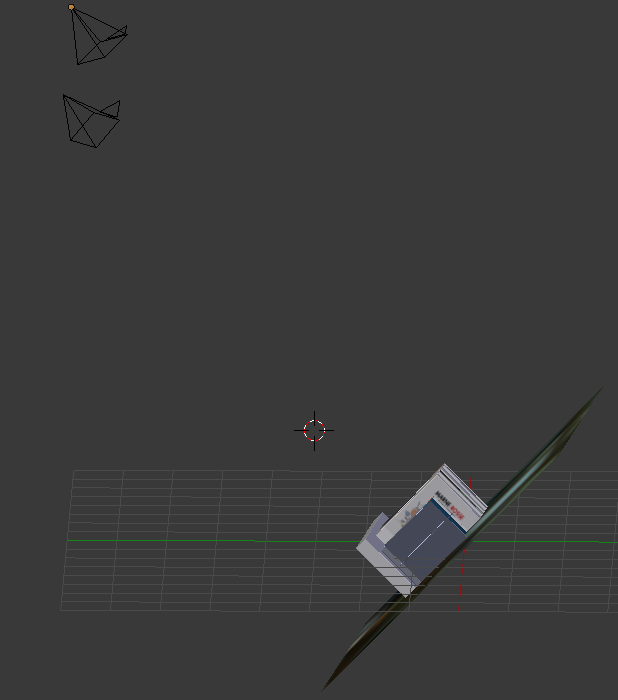
\includegraphics[width=\textwidth]{images/blender3}
                \caption{Right view of our 3D scene.}
                \label{fig:blender1}
        \end{subfigure}
        \begin{subfigure}[b]{0.32\textwidth}
                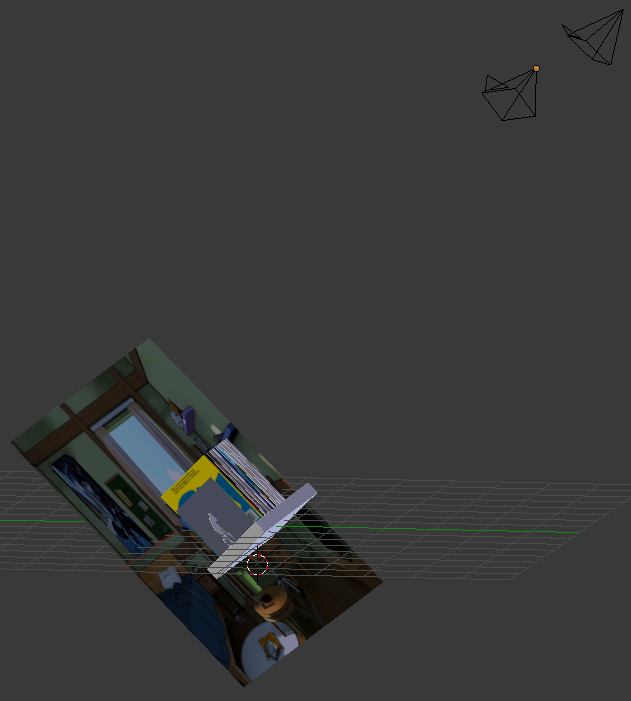
\includegraphics[width=\textwidth]{images/blender6}
                \caption{Left view of our 3D scene.}
                \label{fig:blender2}
        \end{subfigure}
        \begin{subfigure}[b]{0.55\textwidth}
                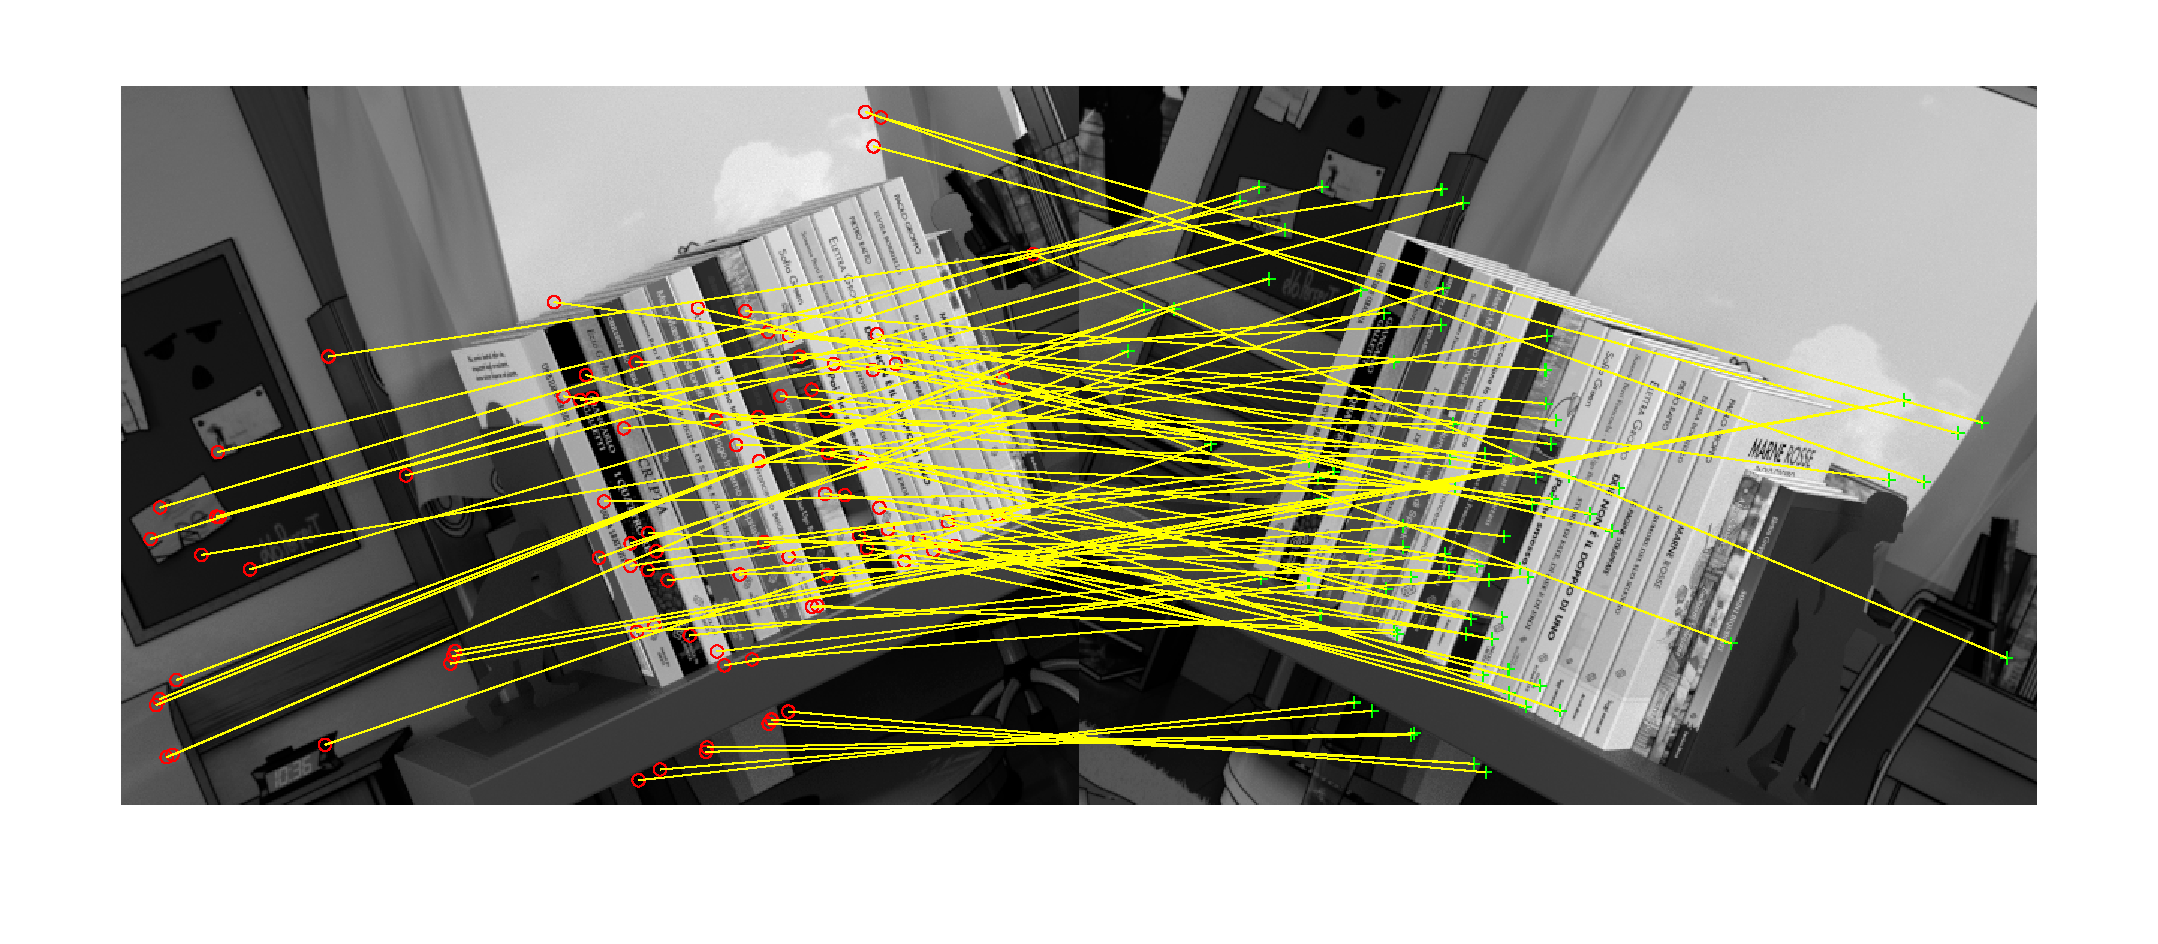
\includegraphics[width=\textwidth]{images/reconstructionMatching}
                \caption{Keypoints matching from each camera view.}
                \label{fig:stereoMatching}
        \end{subfigure}
        \begin{subfigure}[b]{0.45\textwidth}
                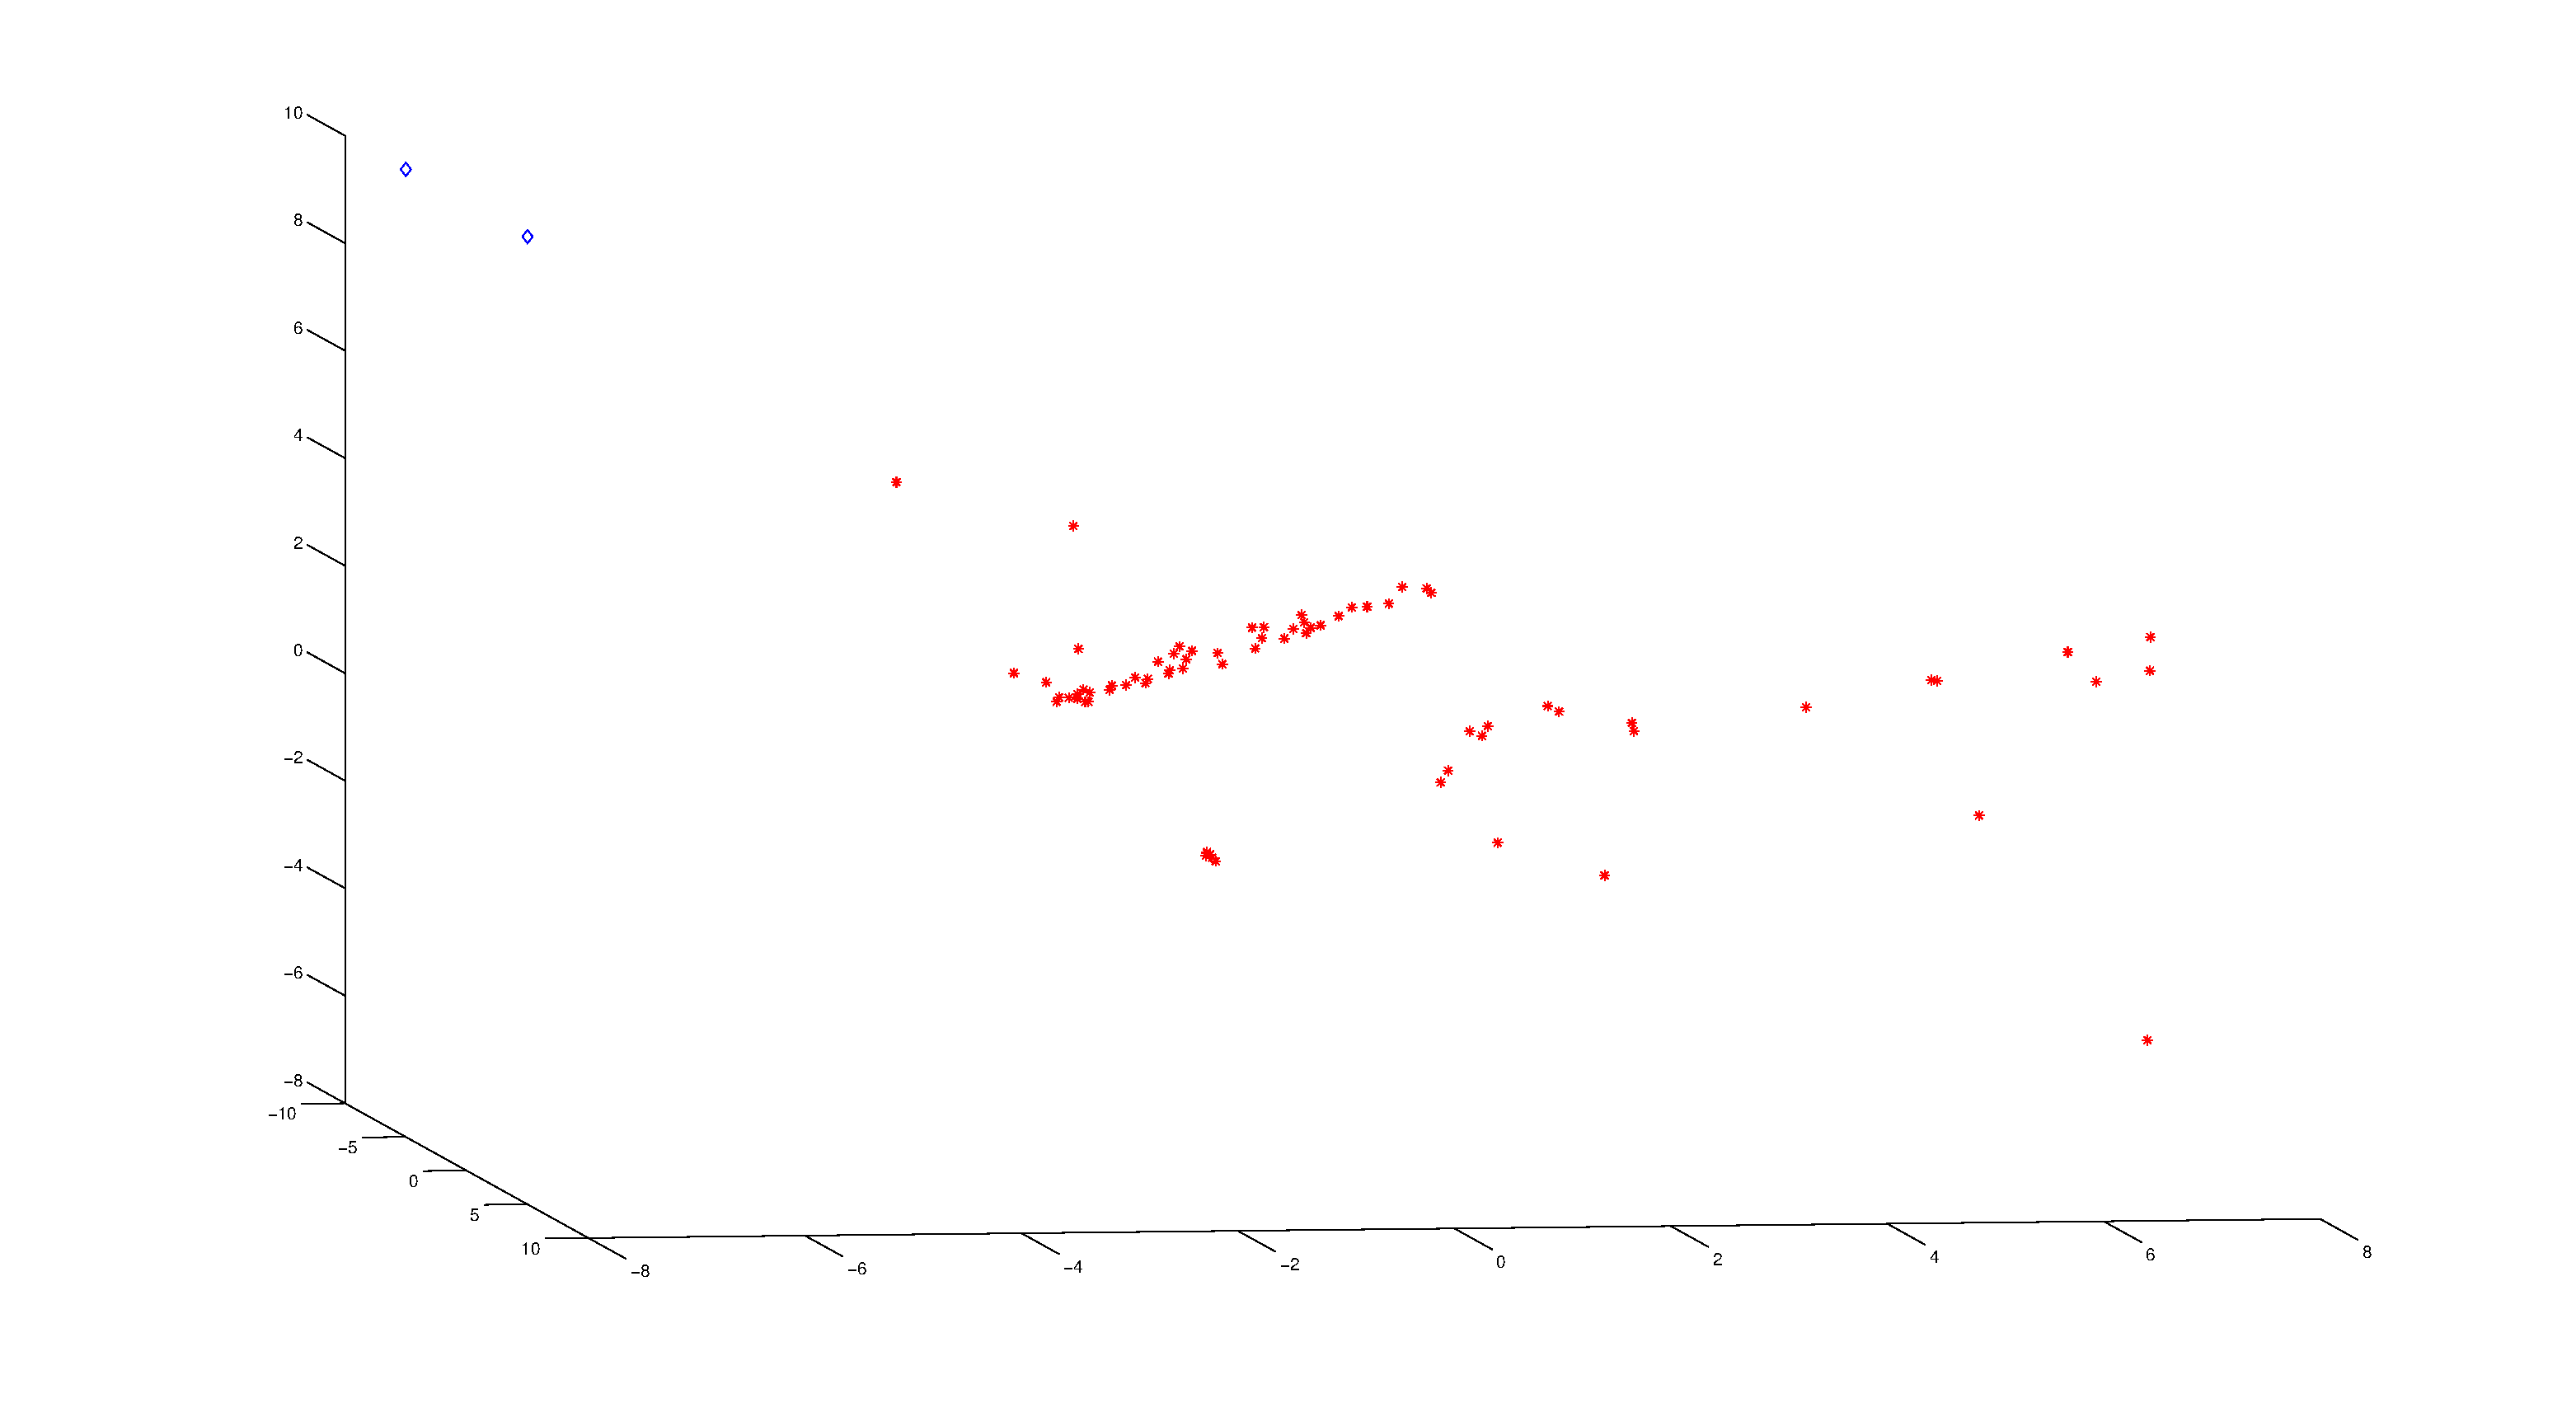
\includegraphics[width=\textwidth]{images/reconstruction1}
                \caption{Right view of the reconstructed points.}
                \label{fig:stereoRecons1}
        \end{subfigure}
        \begin{subfigure}[b]{0.45\textwidth}
                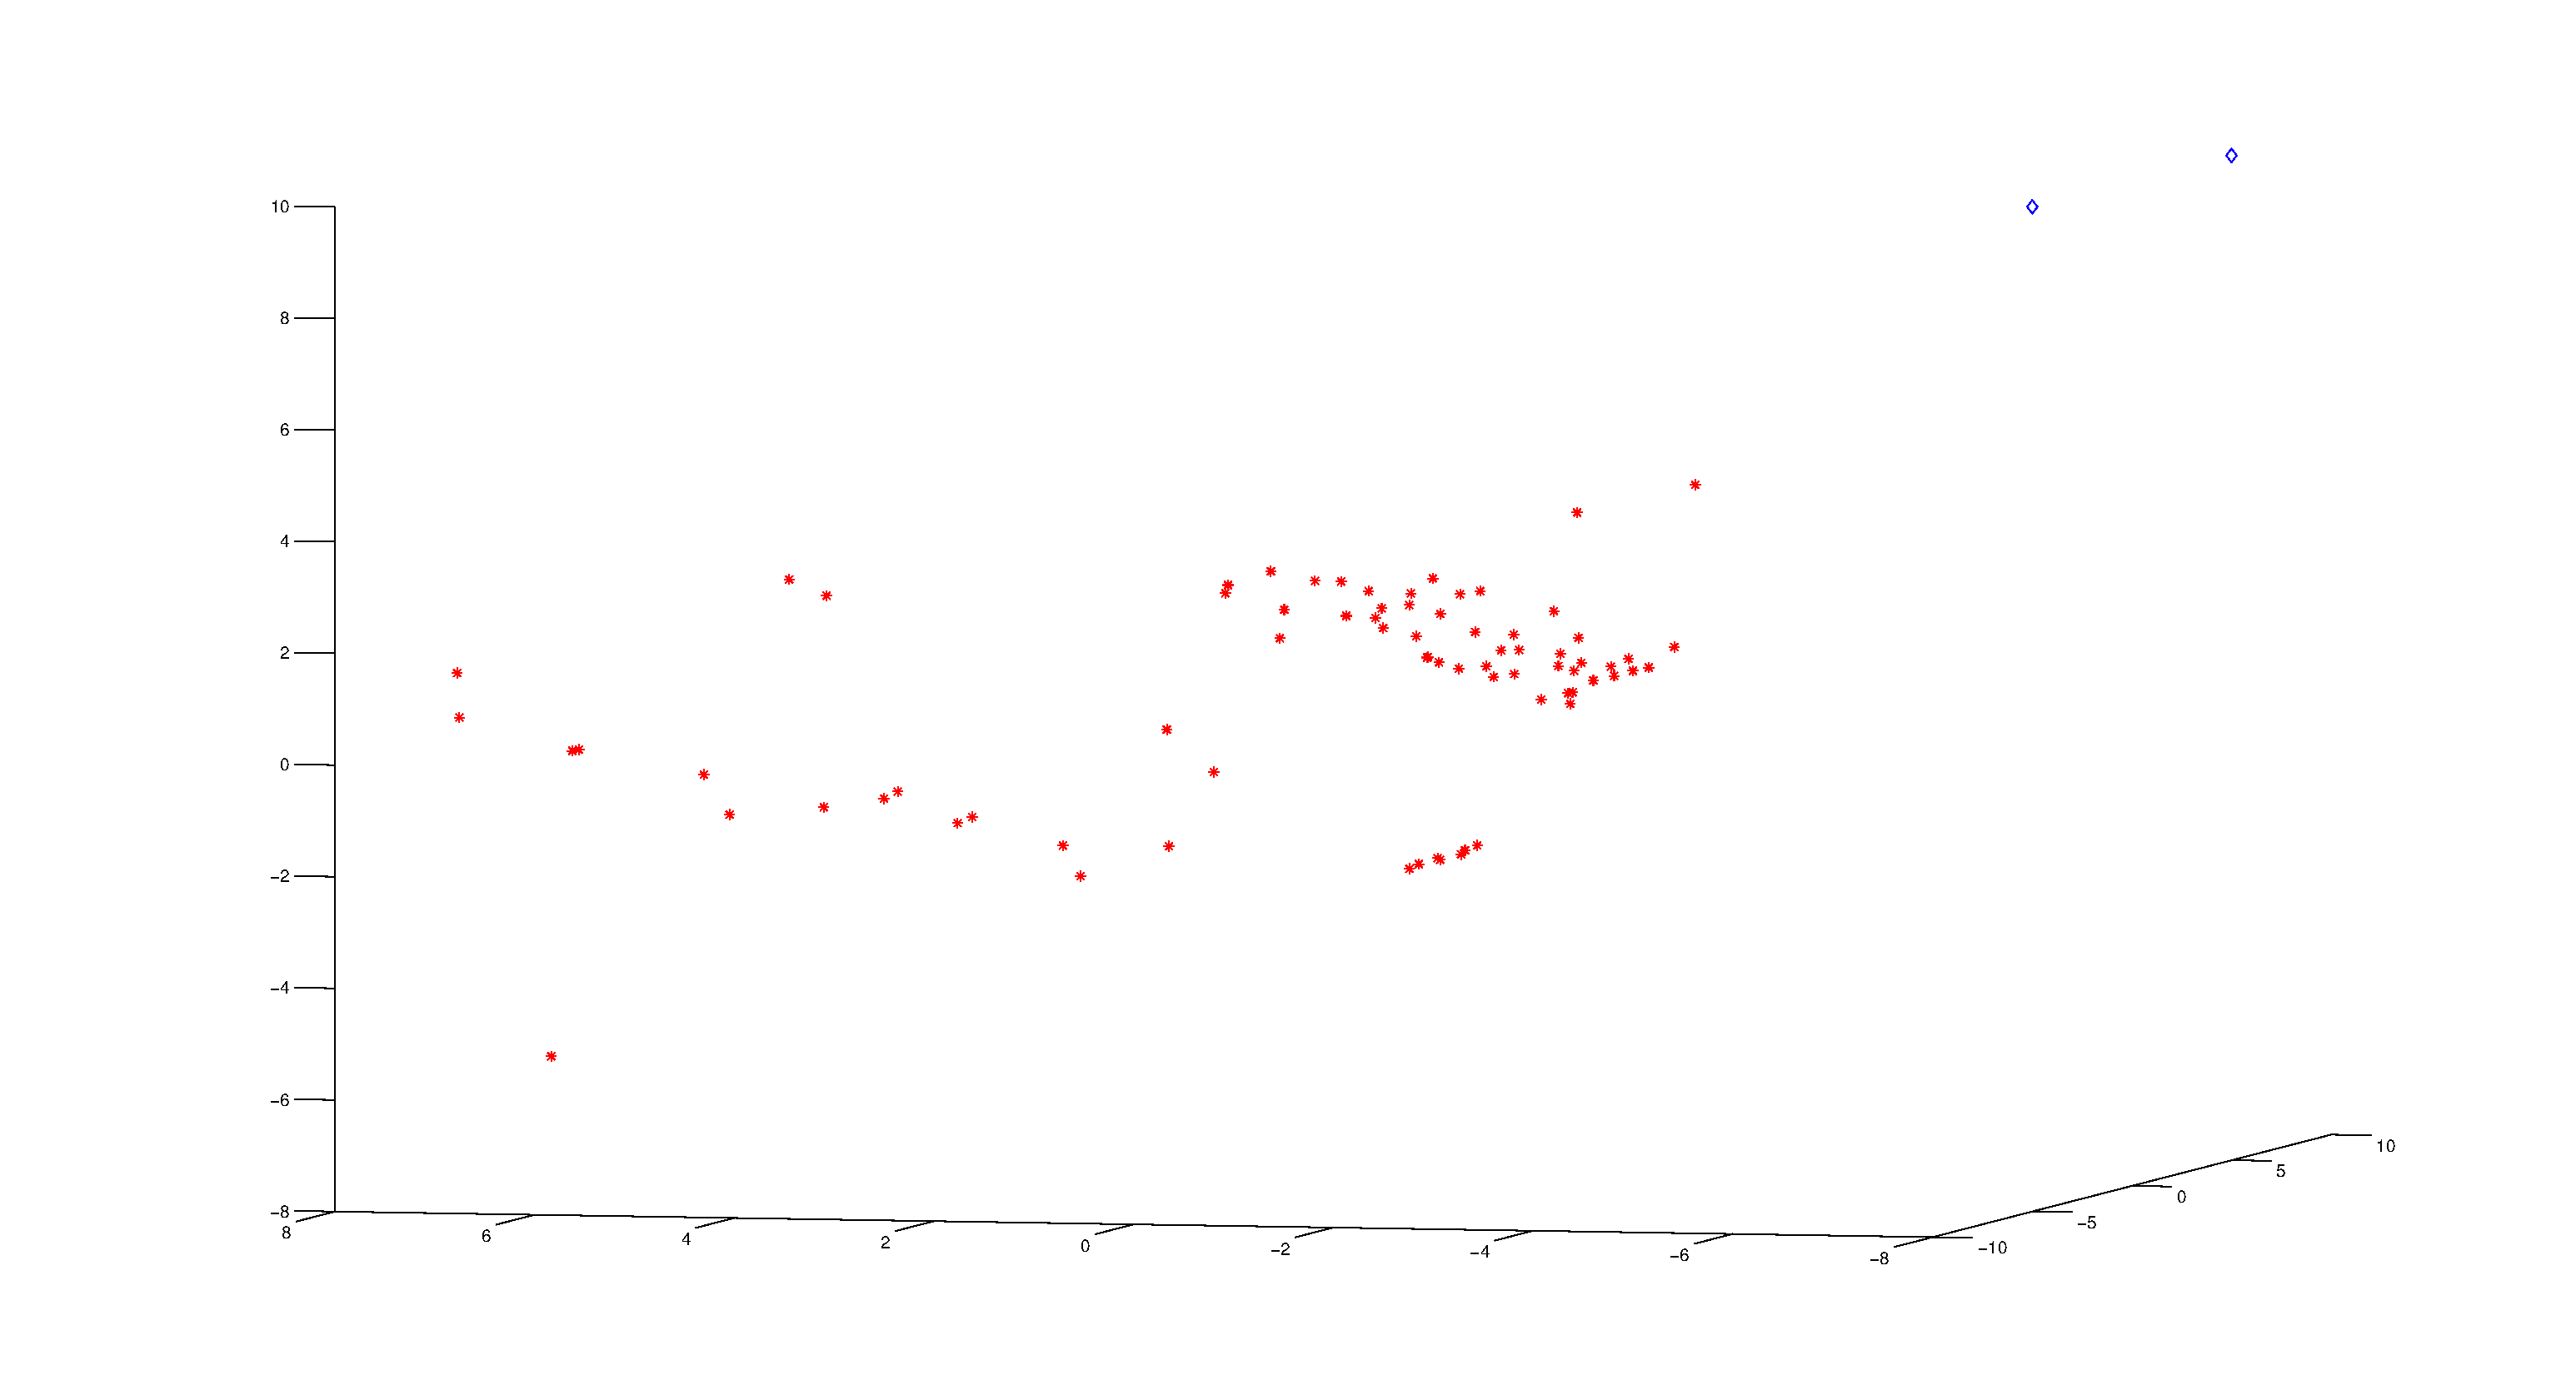
\includegraphics[width=\textwidth]{images/reconstruction3}
                \caption{Left view of the reconstructed points.}
                \label{fig:stereoRecons2}
        \end{subfigure}
        \begin{subfigure}[b]{0.45\textwidth}
                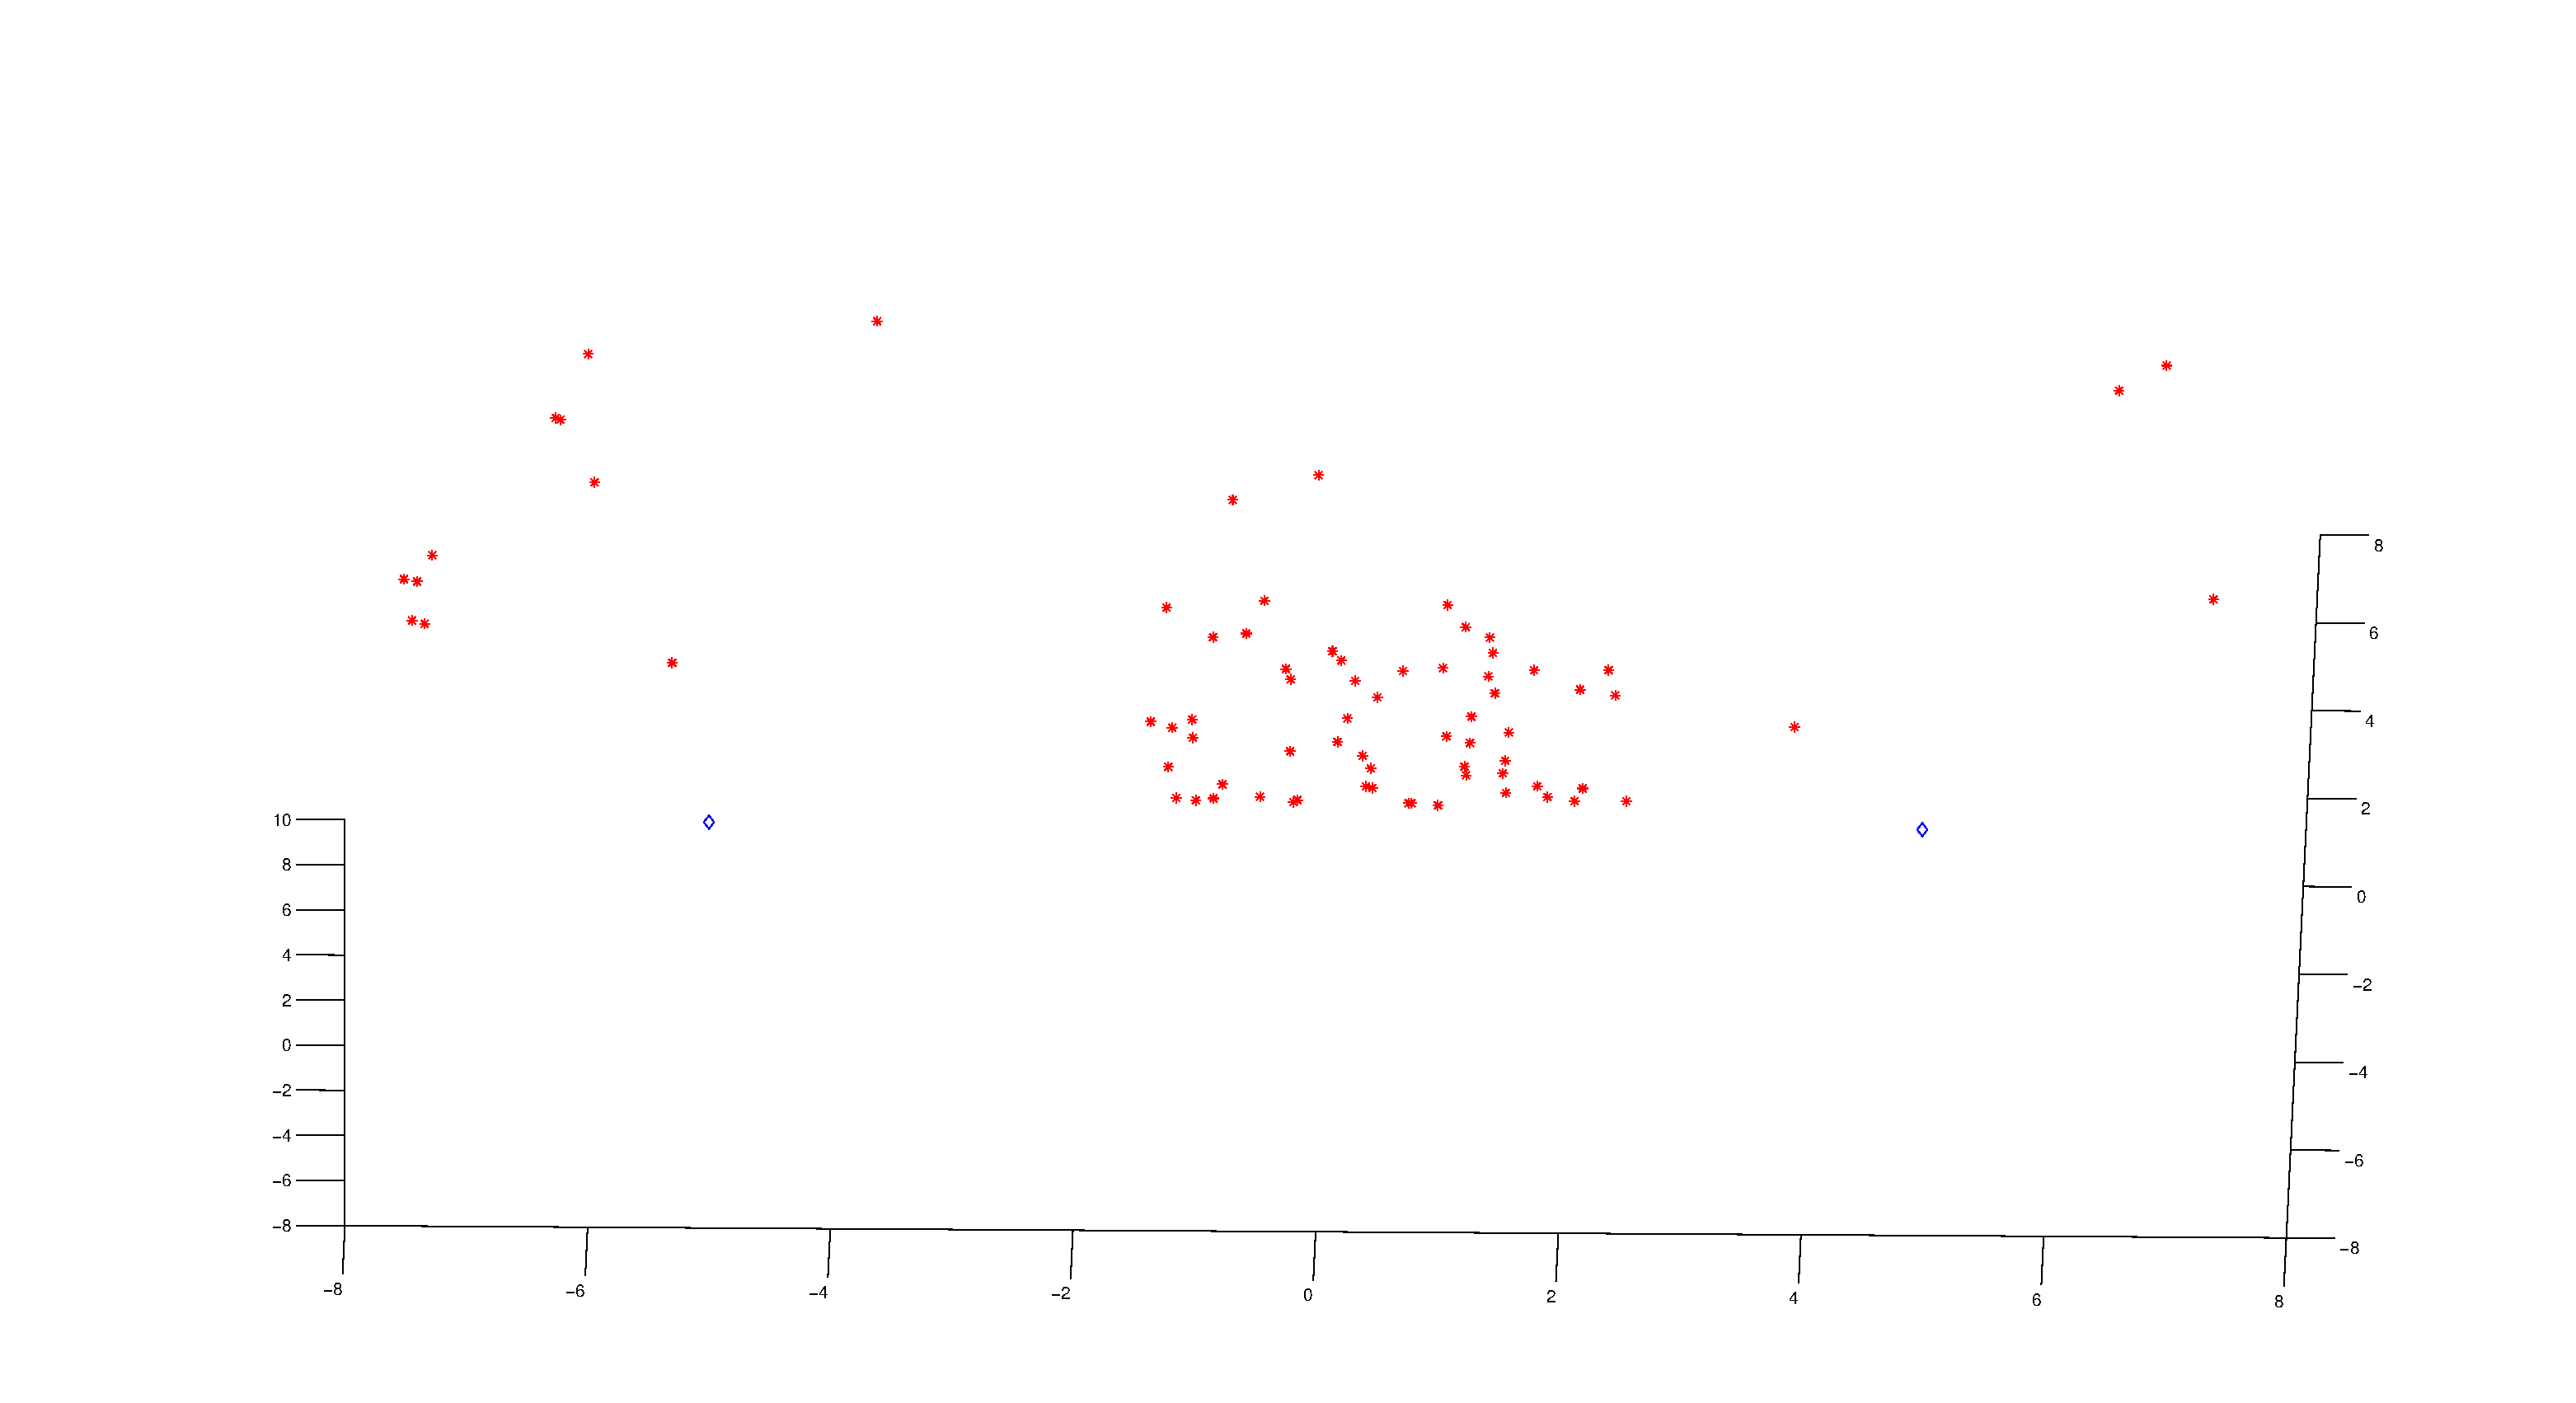
\includegraphics[width=\textwidth]{images/reconstruction2}
                \caption{Central view of the reconstructed points.}
                \label{fig:stereoRecons3}
        \end{subfigure}
        \caption{Reconstructing 3D geometry from a simple scene with books on a shelf.}\label{fig:stereoReconstruction}
\end{figure}

\FloatBarrier
\section{Conclusion and future work}

We have presented the mathematical derivations and algorithm implementations for convolution, keypoint feature detection, image matching, camera calibration and 3D stereo reconstruction.
The next steps would be centred on improving the stereo reconstruction.
In order to achieve a denser reconstruction more points have to be matched, a simple approach to this is to calculate epipolar lines of matching points and then do a neighbour pixel search along that line.
Furthermore, to overcome distortions in the cameras and inherent errors in the numeric methods that are use to calibrate them, the epipolar lines can be forced to be horizontal; and recalibration can be done based on matching information.

\bibliographystyle{apalike}
\bibliography{vuBib}

\end{document}